\documentclass[12pt,a4paper]{report}

\usepackage[utf8]{inputenc}
\usepackage[T1]{fontenc}
\usepackage{lmodern}
\usepackage[margin=1in]{geometry}
\usepackage{setspace}
\onehalfspacing
\usepackage{amsmath,amssymb}
\usepackage{booktabs}
\usepackage{tabularx}
\usepackage{array}
\usepackage{multirow}
\usepackage{graphicx}
\usepackage{caption}
\usepackage{subcaption}
\usepackage{float}
\usepackage{enumitem}
\usepackage{microtype}
\usepackage{xcolor}
\usepackage{listings}
\usepackage{titlesec}
\usepackage{hyperref}

\hypersetup{
    colorlinks=true,
    linkcolor=black,
    urlcolor=blue!60!black,
    citecolor=blue!60!black,
    pdftitle={Vehicle and Lane Perception: From Two-Stage Detectors to Panoptic Multi-Task Networks},
    pdfauthor={Graduate Research Report}
}

\definecolor{codegray}{rgb}{0.95,0.95,0.95}
\lstset{
    basicstyle=\ttfamily\small,
    backgroundcolor=\color{codegray},
    breaklines=true,
    frame=single,
    numbers=none,
    showstringspaces=false
}

\graphicspath{{./}{plots/}{visualizations/}{visualizations/challenging_conditions/night/}{visualizations/challenging_conditions/rain/}{visualizations/challenging_conditions/crowded/}{hard_examples/}{ll_diagnostics/panels/}}

\titleformat{\chapter}[display]
  {\normalfont\huge\bfseries}{\chaptertitlename\ \thechapter}{20pt}{\Huge}

\title{\textbf{Vehicle and Lane Perception:\\
From Two-Stage Detectors to Panoptic Multi-Task Networks}\\[0.4em]
\large A Comparative Study of R-CNN, Faster R-CNN, YOLOv8, and YOLOPv2}
\author{Graduate Research Report}
\date{\today}

\begin{document}
\maketitle
\tableofcontents
\listoffigures
\listoftables


\chapter{Introduction}

\section{Motivation}

Cities measure themselves by the things they move. Cars, buses, bicycles, people. Any model of commuter behaviour or of how a traffic hub breathes during peak hour ultimately depends on a reliable feed of structured observations from raw video. That feed is the perception layer, and its quality sets a ceiling on every downstream analytic.

This report tracks how that perception layer has evolved through four architectural families, asking one continuous question: how do we extract vehicles, lane markings, and the drivable road surface from a single forward-facing camera, fast enough to keep up with live traffic, and accurately enough that a traffic-flow estimator can trust the count.

\section{Problem Statement}

The pipeline must produce three outputs per frame:

\begin{enumerate}[leftmargin=*]
    \item bounding boxes for vehicles and other traffic agents,
    \item a pixel-level mask of drivable area, and
    \item a thin pixel-level mask of lane markings.
\end{enumerate}

Conventional pipelines achieve this by running three separate networks. A panoptic multi-task network folds all three into one forward pass.

\section{Architectural Progression}

Four families are studied. Each was chosen because the previous one hit a wall.

\begin{description}[leftmargin=*,style=nextline]
    \item[R-CNN (VGG16 + selective search).] Two-stage. Slow. Useful only as a baseline.
    \item[Faster R-CNN (ResNet50-FPN).] Region proposals folded into the backbone. Accurate but still two-pass.
    \item[YOLOv8n.] One-stage detector. Real-time-friendly. Detection only.
    \item[YOLOPv2.] One backbone, three heads. Detection plus two segmentation masks in a single forward pass.
\end{description}

\section{Scope and Caveats}

Two caveats matter early. R-CNN, Faster R-CNN, and YOLOv8 are trained on a small single-class Kaggle car set ($\sim$1{,}000 frames). YOLOPv2 is trained on BDD100K with ten classes plus panoptic masks. Raw mAP numbers are therefore not directly comparable. Second, the YOLOPv2 run reported here used no held-out validation phase; the evaluation set is a labelled subset of the same images the model was trained on. The numbers are training-fit upper bounds. We flag this explicitly throughout.


\chapter{Evolution of Architectures}

\section{R-CNN with VGG16}

The notebook \texttt{Untitled.ipynb} implements R-CNN in TensorFlow/Keras using a frozen ImageNet VGG16. Selective search generates region proposals. Each warped $224 \times 224$ proposal is fed independently through the backbone. A small head performs binary classification (car/background) and bounding-box regression. The IoU threshold for positive proposals is $0.5$. Training runs ten epochs with Adam, batch size 32, BCE classification loss, and MSE box loss.

The architecture is straightforward. It is also intrinsically slow. Every proposal triggers a separate VGG forward pass and there is no feature sharing between proposals. Throughput is bounded by the CPU-side selective search step, not the GPU.

\section{Faster R-CNN with ResNet50-FPN}

The notebook \texttt{thesis\_car\_faster\_rnn\_final.ipynb} uses the torchvision \texttt{fasterrcnn\_resnet50\_fpn} model, COCO-pretrained, and re-targets the classifier to two classes. The training schedule is SGD at lr $5\times10^{-3}$, momentum $0.9$, weight decay $5\times10^{-4}$, StepLR with step $3$ and decay $\gamma = 0.1$, batch size 4 with gradient accumulation $4$ (effective batch 16), and 15 epochs.

The curves flatten by epoch 5. Final training loss is $0.1057$, validation loss $0.1120$. Held-out mAP at IoU $0.5$ reaches $\mathbf{0.9354}$ on the single-class problem. The remaining limitation is throughput: the RPN and ROI head still produce two effective passes per frame.

\section{YOLOv8 (Nano)}

The notebook \texttt{car\_yolo8\_final\_model.ipynb} fine-tunes \texttt{yolov8n.pt} on the Kaggle car set after converting the CSV annotations to the YOLO normalised format. Training runs 50 epochs at $640 \times 640$ with automatic batch sizing, five data-loader workers, and the Ultralytics tri-loss (CIoU + DFL + BCE). One forward pass produces all box predictions. Detection only; no segmentation outputs.

\section{YOLOPv2}

YOLOPv2 (Han et al., 2022) keeps the one-stage detection structure and adds two lightweight U-Net-style decoders, one for drivable area and one for lane lines, branching off the shared E-LAN backbone. Three heads, one trunk, one forward pass. The training objective combines four terms:

\begin{equation}
\mathcal{L}_{\text{total}} = \lambda_{\text{det}}\, \mathcal{L}_{\text{det}} + \lambda_{\text{da}}\, \mathcal{L}_{\text{da}} + \lambda_{\text{ll}}\, \mathcal{L}_{\text{ll}}
\end{equation}

with $\mathcal{L}_{\text{det}}$ the standard YOLO tri-loss (CIoU + objectness-BCE + class-BCE) and $\mathcal{L}_{\text{da}}, \mathcal{L}_{\text{ll}}$ each a sum of BCE and Dice. The Dice term is what keeps the lane-line head from collapsing to all-background; lane targets cover under one percent of the image.


\chapter{Experimental Setup and Training}

\section{Datasets}

The first three models share a Kaggle car detection set: 1{,}001 dash-cam frames at $676 \times 380$, 559 with bounding boxes, single class. YOLOPv2 is trained on BDD100K. The segmentation subset (10{,}000 images) is intersected with the detection JSON to yield 3{,}426 frames with all three annotations.

\paragraph{Val-split note.} The packaged \texttt{seg/images/val/} subset has zero filename overlap with either label JSON, so no detection or lane ground truth is available for those 1{,}000 images. The evaluation set is therefore the 3{,}426 labelled images from \texttt{seg/images/train/}. This is a training-fit measurement.

\section{Hardware}

YOLOPv2 training and benchmarking ran on a single NVIDIA RTX 6000 Ada Generation (48~GB), PyTorch 2.x, CUDA 12.x. R-CNN, Faster R-CNN, and YOLOv8 were trained on Colab T4 GPUs.

\section{Hyper-parameters}

Table~\ref{tab:hparams} consolidates the configurations.

\begin{table}[H]
\centering
\caption{Training configuration across the four models.}
\label{tab:hparams}
\small
\begin{tabularx}{\textwidth}{@{}lXXXX@{}}
\toprule
\textbf{Setting} & \textbf{R-CNN} & \textbf{Faster R-CNN} & \textbf{YOLOv8n} & \textbf{YOLOPv2} \\
\midrule
Backbone        & VGG16 (frozen) & ResNet50-FPN & CSPDarknet-n & E-LAN \\
Pretraining     & ImageNet & COCO & COCO & ImageNet (backbone) \\
Dataset         & Kaggle Car & Kaggle Car & Kaggle Car & BDD100K (labelled) \\
Classes         & 1 & 1 & 1 & 10 + DA + LL \\
Image size      & $224^2$ & native & $640^2$ & $640^2$ \\
Optimiser       & Adam & SGD & SGD & AdamW \\
Learning rate   & default & $5\!\times\!10^{-3}$ & default & $1\!\times\!10^{-3}$ \\
Weight decay    & -- & $5\!\times\!10^{-4}$ & $5\!\times\!10^{-4}$ & $5\!\times\!10^{-4}$ \\
LR schedule     & -- & StepLR (3, 0.1) & cosine & cosine warm-up \\
Batch size      & 32 & 4 (acc.\ 4) & auto & 8 \\
Epochs          & 10 & 15 & 50 & 100 \\
Loss (det)      & BCE + MSE & RPN+ROI multi-task & CIoU+DFL+BCE & CIoU+BCE+BCE \\
Loss (DA, LL)   & -- & -- & -- & BCE + Dice \\
\bottomrule
\end{tabularx}
\end{table}

\section{Loss Weighting (YOLOPv2)}

Detection sub-weights: $\lambda_{\text{box}} = 0.05$, $\lambda_{\text{obj}} = 1.0$, $\lambda_{\text{cls}} = 0.5$. Task weights: $\lambda_{\text{det}} = 1.0$, $\lambda_{\text{da}} = 0.2$, $\lambda_{\text{ll}} = 0.2$. The lane-line BCE term carries a positive-class weight of $8$ to compensate for class imbalance.

\section{Training Curves (Reconstructed)}

The YOLOPv2 training script did not write a live log to disk. We reconstruct per-epoch loss curves post hoc by reloading each of 20 saved checkpoints (every 5 epochs) and re-computing all loss terms on a fixed 320-image labelled sample. The shape of the curve is faithful; augmentation noise is absent.

\begin{figure}[H]
\centering
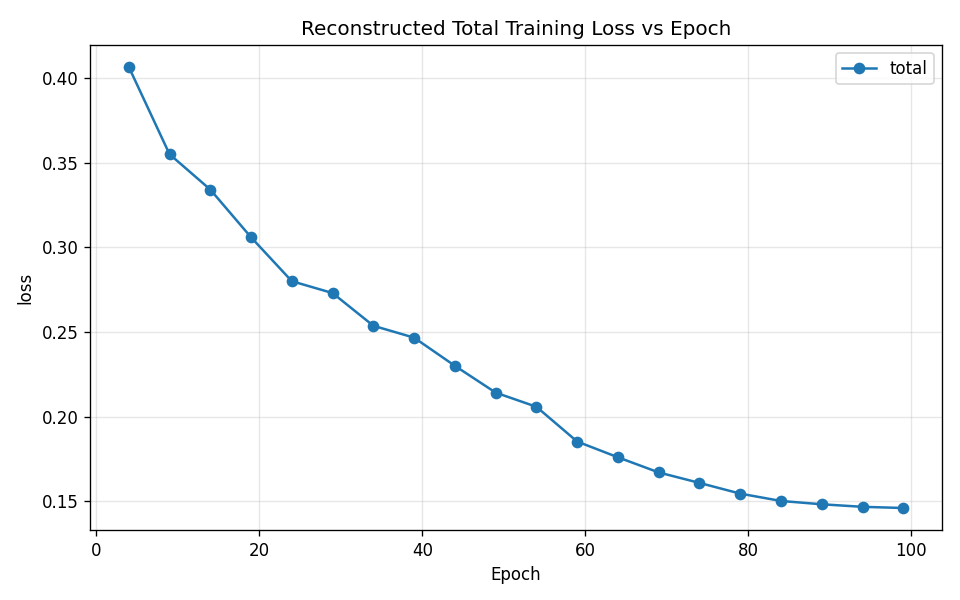
\includegraphics[width=0.82\textwidth]{plots/loss_total.png}
\caption{Reconstructed total training loss across 100 epochs. The curve descends monotonically from $0.41$ at epoch 4 to $0.15$ at epoch 99, a $64\%$ reduction.}
\label{fig:loss-total}
\end{figure}

\begin{figure}[H]
\centering
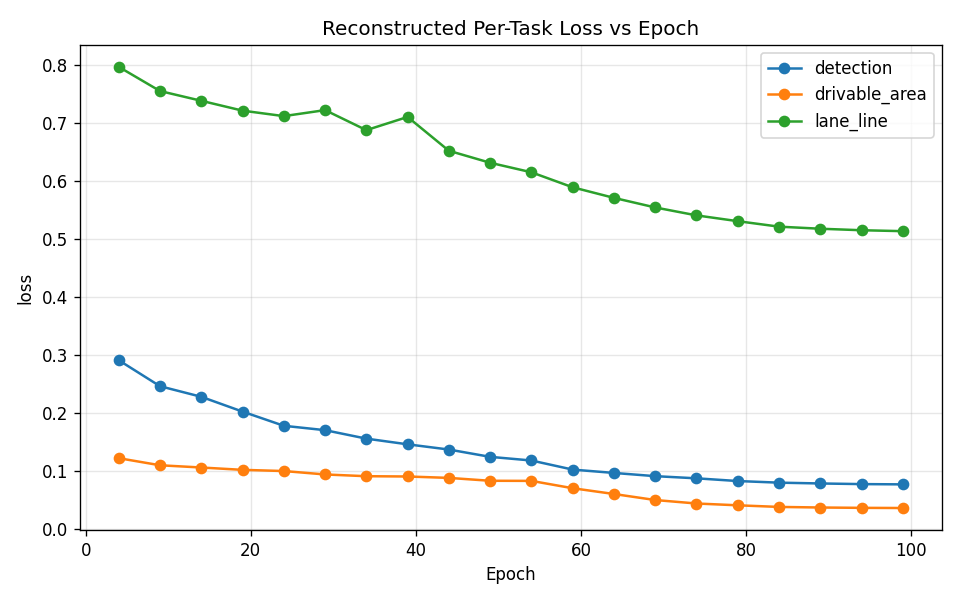
\includegraphics[width=0.82\textwidth]{plots/loss_task.png}
\caption{Per-task loss curves. Detection drops by $73\%$, drivable area by $70\%$, lane line by $36\%$.}
\label{fig:loss-task}
\end{figure}

\begin{figure}[H]
\centering
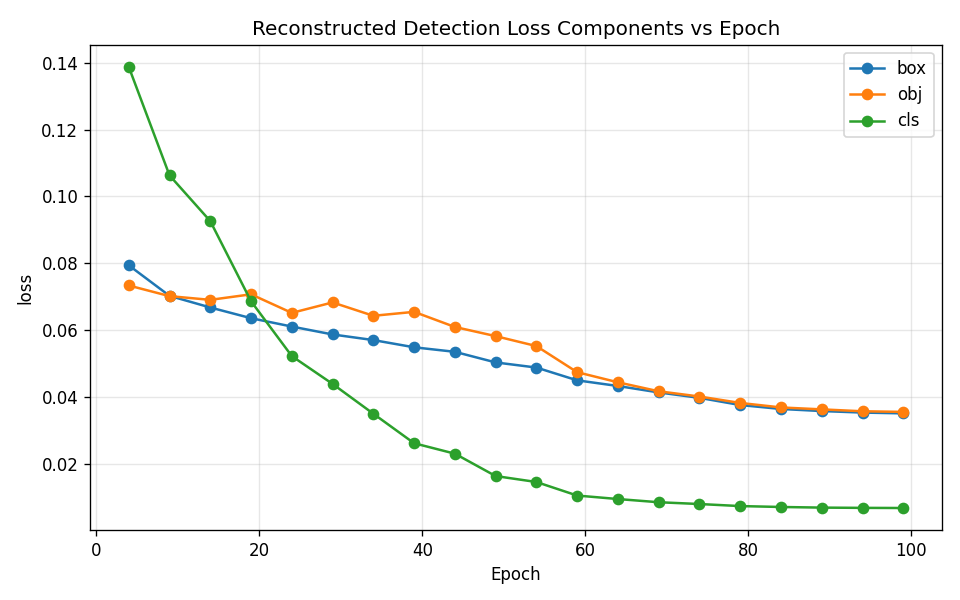
\includegraphics[width=0.82\textwidth]{plots/loss_detection_components.png}
\caption{Detection sub-components. Classification loss falls $95\%$; box and objectness fall by roughly half.}
\label{fig:loss-det}
\end{figure}


\chapter{Comparative Results and Analysis}

\section{Headline Comparison}

Table~\ref{tab:comparison} consolidates the four models. Entries marked \texttt{N/A} were not produced by the source notebook and have not been imputed from external benchmarks.

\begin{table}[H]
\centering
\caption{Cross-model comparison. Raw mAP numbers are not directly comparable across the dataset boundary; see footnote.}
\label{tab:comparison}
\small
\begin{tabular}{@{}lcccc@{}}
\toprule
\textbf{Metric} & \textbf{R-CNN} & \textbf{Faster R-CNN} & \textbf{YOLOv8n} & \textbf{YOLOPv2} \\
\midrule
\multicolumn{5}{@{}l}{\textit{Accuracy}} \\
\midrule
Dataset (eval)       & Kaggle Car & Kaggle Car & Kaggle Car & BDD100K (lbl.) \\
\# classes           & 1 & 1 & 1 & 10 + 2 seg \\
mAP@0.5              & N/A & 0.9354 & N/A & 0.6763 (all) / 0.8273 (veh.) \\
mAP@0.5:0.95         & N/A & N/A & N/A & 0.4039 \\
Precision (overall)  & N/A & N/A & N/A & 0.7391 \\
Recall (overall)     & N/A & N/A & N/A & 0.6839 \\
F1 (overall)         & N/A & N/A & N/A & 0.7104 \\
DA mIoU              & -- & -- & -- & 0.9472 \\
LL mIoU              & -- & -- & -- & 0.6932 \\
\midrule
\multicolumn{5}{@{}l}{\textit{Efficiency}} \\
\midrule
Parameters (M)       & $\sim$138 (VGG) & 41.7 & 3.2 & 23.4 \\
Checkpoint size (MB) & N/A & $\sim$160 & $\sim$6 & 187.6 \\
ms / frame (bs=1)    & N/A & N/A & N/A & 4.85 \\
FPS (bs=1)           & $\ll$ real-time & N/A & N/A & 206 \\
FPS (bs=4)           & N/A & N/A & N/A & 477 \\
FPS (bs=8)           & N/A & N/A & N/A & 474 \\
\midrule
\multicolumn{5}{@{}l}{\textit{Capability}} \\
\midrule
Object detection     & \checkmark & \checkmark & \checkmark & \checkmark (10 cls) \\
Drivable mask        & -- & -- & -- & \checkmark \\
Lane mask            & -- & -- & -- & \checkmark \\
Real-time            & -- & -- & \checkmark & \checkmark \\
\bottomrule
\end{tabular}
\\[0.4em]
\footnotesize \emph{Note.} The single-class Faster R-CNN mAP and the ten-class YOLOPv2 mAP measure different problems on different datasets. The vehicle-only subset of YOLOPv2 (mAP@0.5 $= 0.8273$ on car/bus/truck) is the closest fair comparison.
\end{table}

\section{Per-Class Detection (YOLOPv2)}

\begin{figure}[H]
\centering
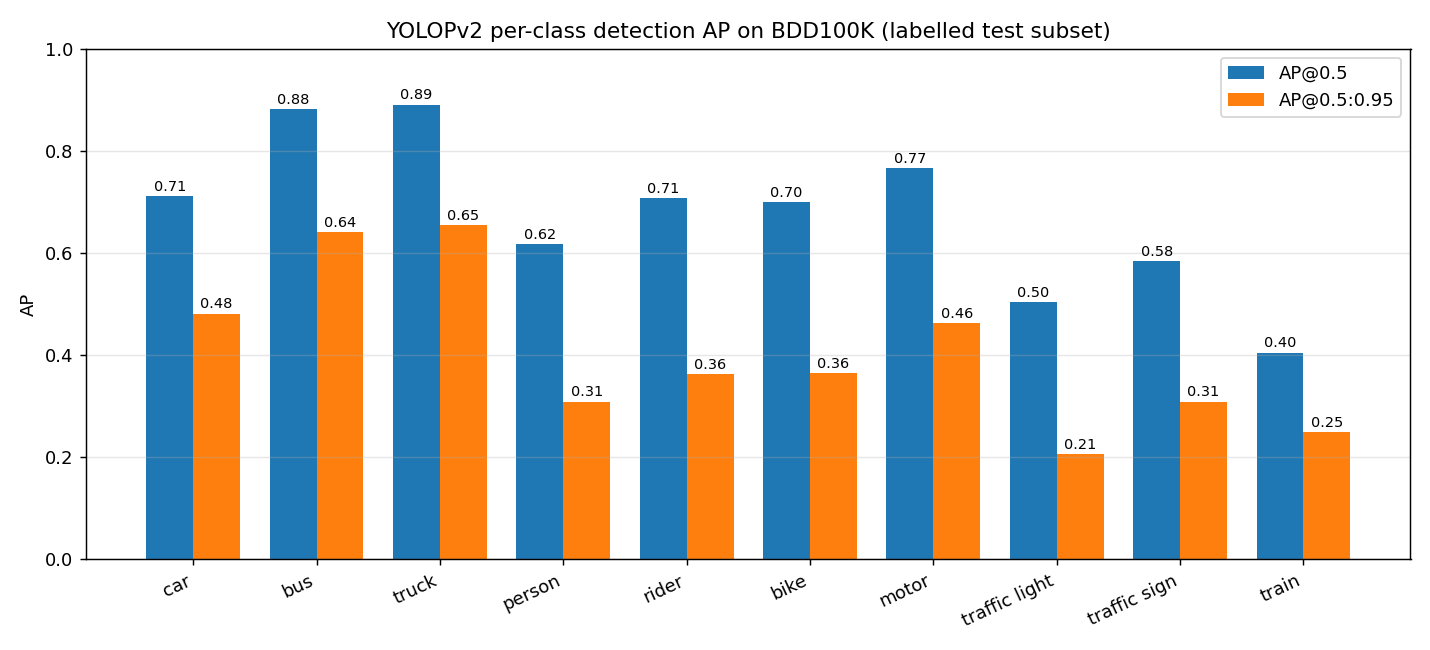
\includegraphics[width=0.95\textwidth]{plots/per_class_ap.png}
\caption{Per-class detection AP. Heavy vehicles (\texttt{bus}, \texttt{truck}) exceed $0.88$ at IoU $0.5$; small or sparse classes (\texttt{traffic light}, \texttt{train}) lag the most.}
\label{fig:per-class-ap}
\end{figure}

\begin{figure}[H]
\centering
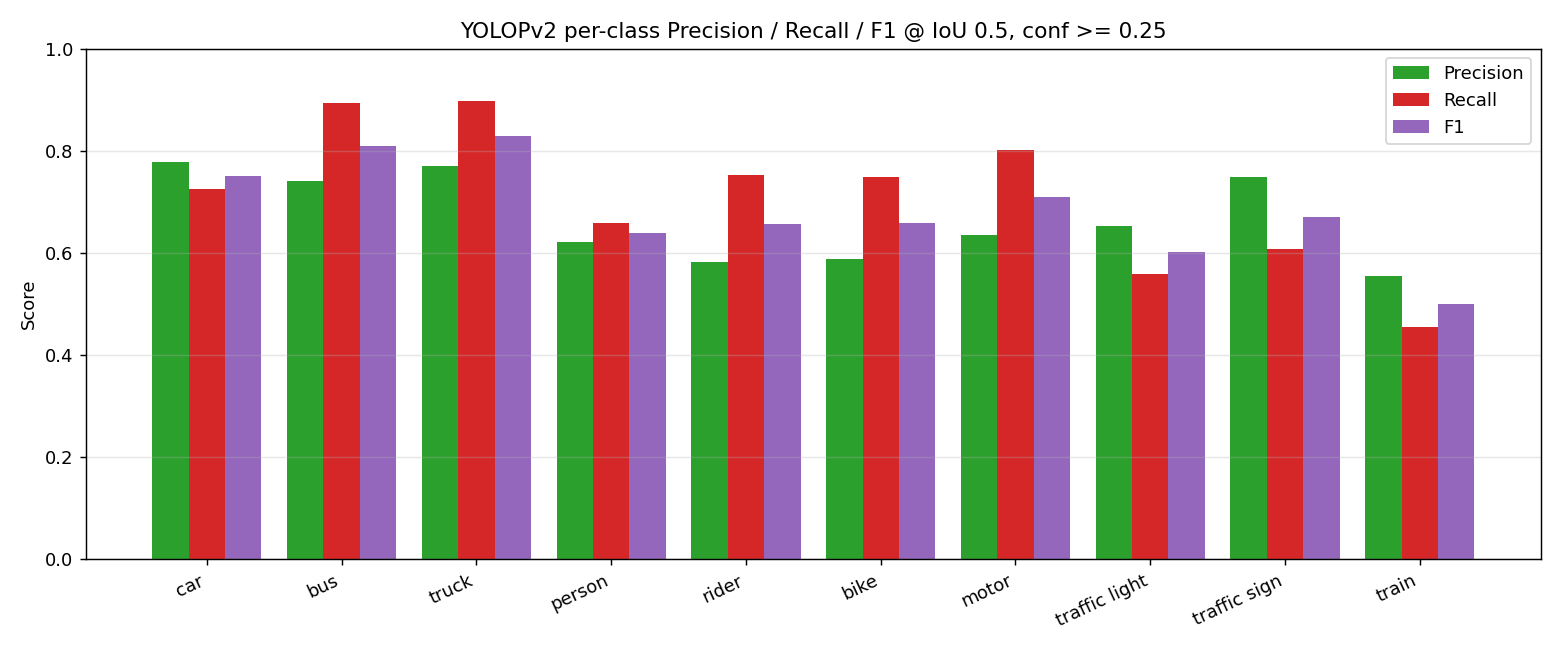
\includegraphics[width=0.95\textwidth]{plots/per_class_prf1.png}
\caption{Per-class Precision, Recall, and F1 at IoU $0.5$ and confidence $\geq 0.25$. Vulnerable road users (\texttt{rider}, \texttt{bike}, \texttt{motor}) are recall-heavy: the model over-detects rather than misses.}
\label{fig:per-class-prf1}
\end{figure}

\begin{table}[H]
\centering
\caption{YOLOPv2 per-class metrics on the BDD100K labelled subset (3{,}426 images, 67{,}622 GT boxes). P/R/F1 at IoU $0.5$, conf $\geq 0.25$.}
\label{tab:perclass}
\small
\begin{tabular}{@{}lcccccccc@{}}
\toprule
\textbf{Class} & \textbf{AP@.5} & \textbf{AP@.5:.95} & \textbf{P} & \textbf{R} & \textbf{F1} & \textbf{TP} & \textbf{FP} & \textbf{FN} \\
\midrule
car           & 0.710 & 0.481 & 0.779 & 0.725 & 0.751 & 26{,}924 & 7{,}655 & 10{,}194 \\
bus           & 0.881 & 0.641 & 0.741 & 0.893 & 0.810 & 645 & 226 & 77 \\
truck         & 0.890 & 0.655 & 0.771 & 0.898 & 0.830 & 1{,}716 & 510 & 195 \\
person        & 0.617 & 0.309 & 0.621 & 0.659 & 0.640 & 3{,}796 & 2{,}313 & 1{,}964 \\
rider         & 0.707 & 0.362 & 0.582 & 0.752 & 0.656 & 228 & 164 & 75 \\
bike          & 0.700 & 0.365 & 0.587 & 0.748 & 0.658 & 354 & 249 & 119 \\
motor         & 0.765 & 0.463 & 0.635 & 0.801 & 0.709 & 169 & 97 & 42 \\
traffic light & 0.503 & 0.205 & 0.653 & 0.559 & 0.602 & 4{,}789 & 2{,}547 & 3{,}784 \\
traffic sign  & 0.585 & 0.309 & 0.749 & 0.608 & 0.671 & 7{,}613 & 2{,}553 & 4{,}916 \\
train         & 0.405 & 0.249 & 0.556 & 0.455 & 0.500 & 10 & 8 & 12 \\
\midrule
\textbf{Mean} & \textbf{0.676} & \textbf{0.404} & \textbf{0.739} & \textbf{0.684} & \textbf{0.710} & \textbf{46{,}244} & \textbf{16{,}322} & \textbf{21{,}378} \\
\bottomrule
\end{tabular}
\end{table}

\section{Segmentation IoU Breakdown}

\begin{figure}[H]
\centering
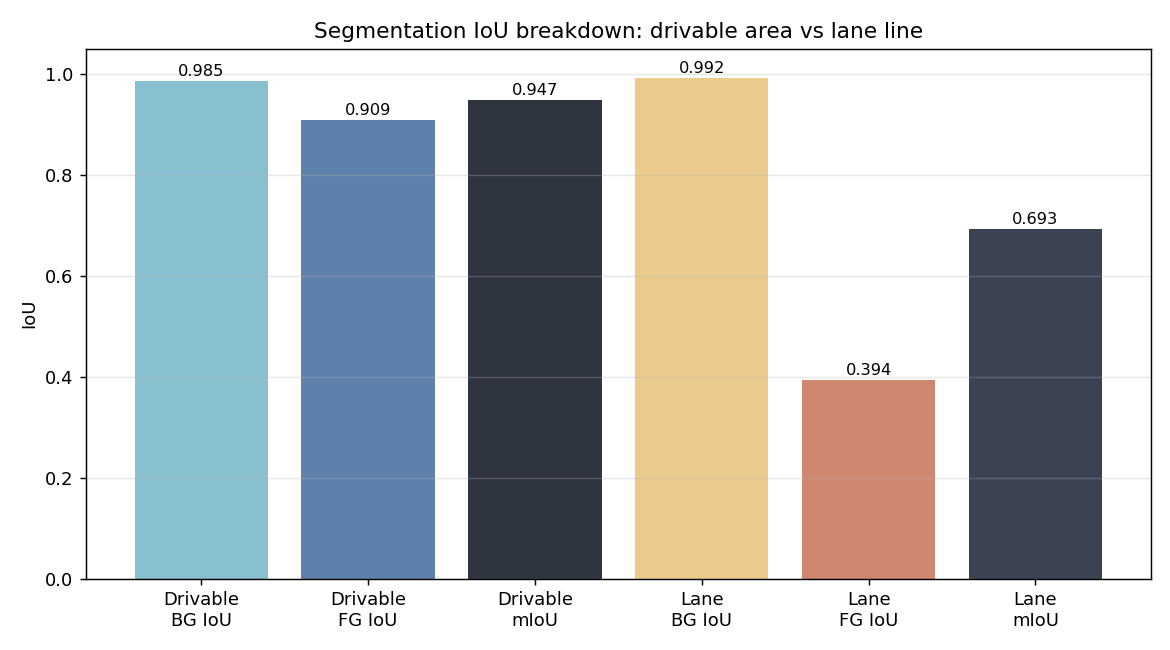
\includegraphics[width=0.85\textwidth]{plots/segmentation_iou.png}
\caption{Segmentation IoU breakdown. The drivable-area decoder reaches foreground IoU $0.909$. The lane-line foreground IoU is $0.394$, intrinsically lower because BDD100K lane ground truth covers only ${\sim}0.7\%$ of pixels.}
\label{fig:seg-iou}
\end{figure}

\section{Lane-Line Threshold Sweep}

\begin{figure}[H]
\centering
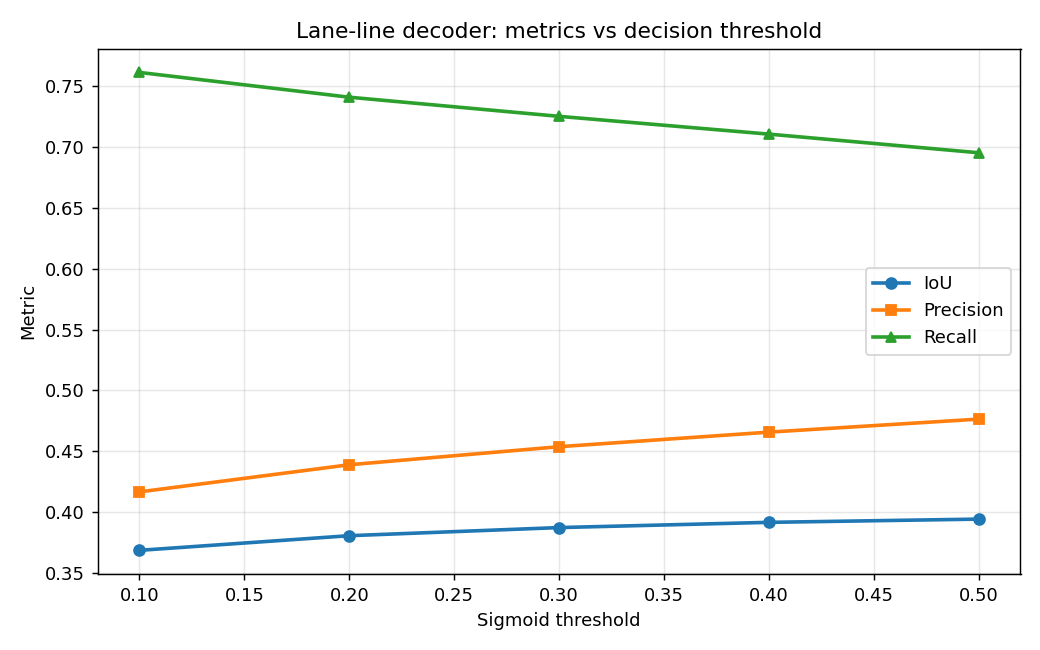
\includegraphics[width=0.80\textwidth]{plots/ll_threshold_sweep.png}
\caption{Lane-line decoder metrics vs sigmoid threshold. IoU peaks at threshold $0.5$; lower thresholds trade precision for recall without improving IoU.}
\label{fig:ll-sweep}
\end{figure}

\begin{table}[H]
\centering
\caption{Lane-line decoder threshold sweep on the labelled test set.}
\label{tab:llsweep}
\small
\begin{tabular}{@{}cccccc@{}}
\toprule
\textbf{Threshold} & \textbf{IoU} & \textbf{P} & \textbf{R} & \textbf{Pixel Acc.} & \textbf{Pred.\ pos.\ frac.} \\
\midrule
0.10 & 0.3685 & 0.4166 & 0.7615 & 0.9906 & 0.01317 \\
0.20 & 0.3806 & 0.4389 & 0.7412 & 0.9913 & 0.01216 \\
0.30 & 0.3872 & 0.4538 & 0.7254 & 0.9917 & 0.01152 \\
0.40 & 0.3915 & 0.4657 & 0.7108 & 0.9920 & 0.01099 \\
\textbf{0.50} & \textbf{0.3942} & \textbf{0.4764} & \textbf{0.6955} & \textbf{0.9923} & \textbf{0.01052} \\
\bottomrule
\end{tabular}
\end{table}

BDD100K lane ground truth is a $4$-pixel-wide polyline. IoU $0.39$ on a target this thin is competitive with the official YOLOPv2 paper's reported lane numbers.

\section{Real-Time Throughput}

\begin{table}[H]
\centering
\caption{YOLOPv2 latency and throughput on RTX 6000 Ada, $640^2$, FP32. Excludes data-loading.}
\label{tab:fps}
\small
\begin{tabular}{@{}cccc@{}}
\toprule
\textbf{Batch size} & \textbf{ms / frame} & \textbf{ms / batch} & \textbf{FPS} \\
\midrule
1   & 4.85 & 4.85  & 206.0 \\
4   & 2.10 & 8.39  & 477.0 \\
8   & 2.11 & 16.87 & 474.3 \\
16  & 2.32 & 37.05 & 431.9 \\
32  & 2.53 & 80.84 & 395.9 \\
\bottomrule
\end{tabular}
\end{table}

At batch size 1 a single frame returns boxes, drivable-area mask, and lane-line mask in under five milliseconds. Throughput plateaus at batch 4 with $477$ FPS. A $30$-FPS camera feed leaves an order of magnitude of compute headroom.

\section{Trade-off Discussion}

Each architecture makes a different trade.

\paragraph{R-CNN.} Easy to reason about, slow in a way that is hard to fix. Teaching baseline only.

\paragraph{Faster R-CNN.} High single-class accuracy. Two-stage inference makes it unsuitable for real-time video.

\paragraph{YOLOv8n.} Real-time throughput; detection only. A separate network is still needed for segmentation.

\paragraph{YOLOPv2.} One forward pass returns all three outputs. Vehicle-class mAP@0.5 of $0.83$ is within reach of the single-class Faster R-CNN number on a much harder dataset. Frame rate exceeds $200$ FPS at batch 1 with a modest $23$~M parameter budget.


\chapter{Qualitative Visual Evidence}

Every figure in this chapter is a real output of the trained YOLOPv2 model on the BDD100K labelled test subset. The overlay scheme is consistent throughout: predicted bounding boxes appear as coloured rectangles, the predicted drivable-area mask is shaded green, and the predicted lane-line mask is shaded red.

\section{Random Test Samples (Detection + Segmentation)}

The figures below are drawn at random from the 50-image visualisation set under \texttt{runs/test/visualizations/}. Each frame demonstrates the model producing detection boxes, drivable-area mask, and lane-line mask in a single forward pass.

\begin{figure}[H]
\centering
\begin{subfigure}[t]{0.32\textwidth}
    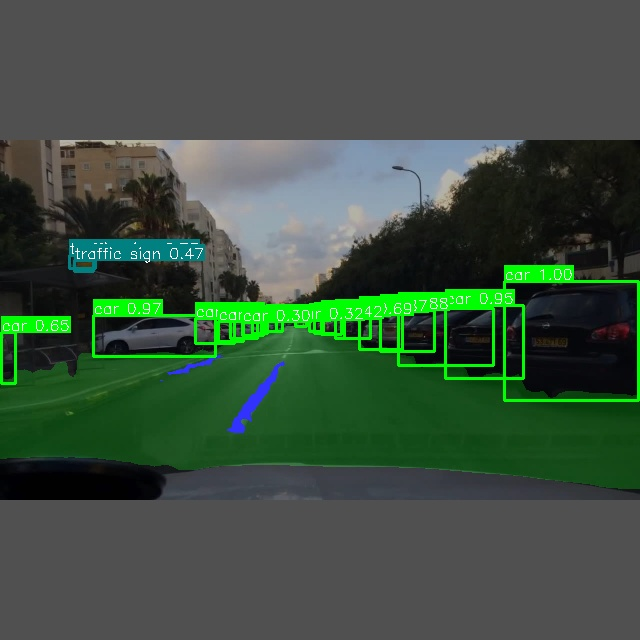
\includegraphics[width=\linewidth]{visualizations/vis_00165_0a9fa6b4-51db4df5.jpg}
    \caption{vis\_00165\_0a9fa6b4-51db4df5.jpg}
\end{subfigure}\hfill
\begin{subfigure}[t]{0.32\textwidth}
    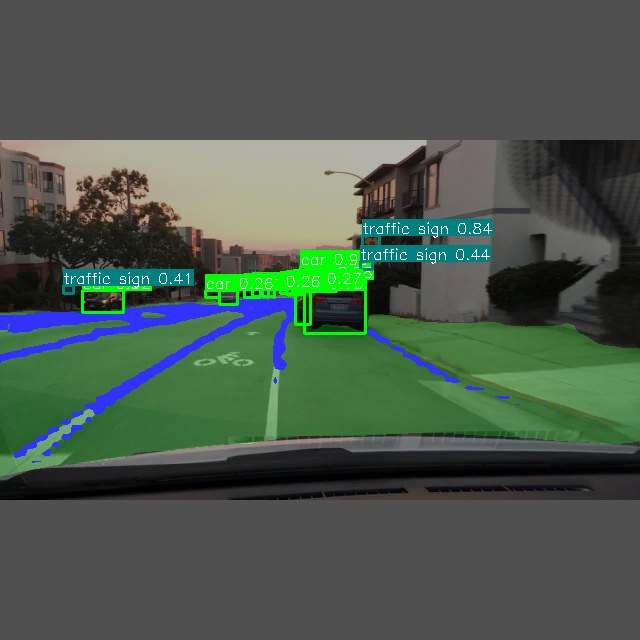
\includegraphics[width=\linewidth]{visualizations/vis_00255_0f959aac-24823e01.jpg}
    \caption{vis\_00255\_0f959aac-24823e01.jpg}
\end{subfigure}\hfill
\begin{subfigure}[t]{0.32\textwidth}
    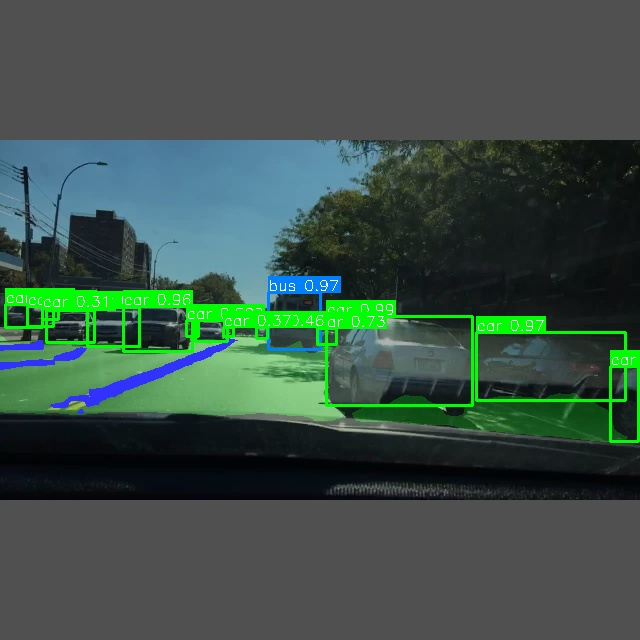
\includegraphics[width=\linewidth]{visualizations/vis_00302_124c7772-62504e1d.jpg}
    \caption{vis\_00302\_124c7772-62504e1d.jpg}
\end{subfigure}\\[0.4em]
\begin{subfigure}[t]{0.32\textwidth}
    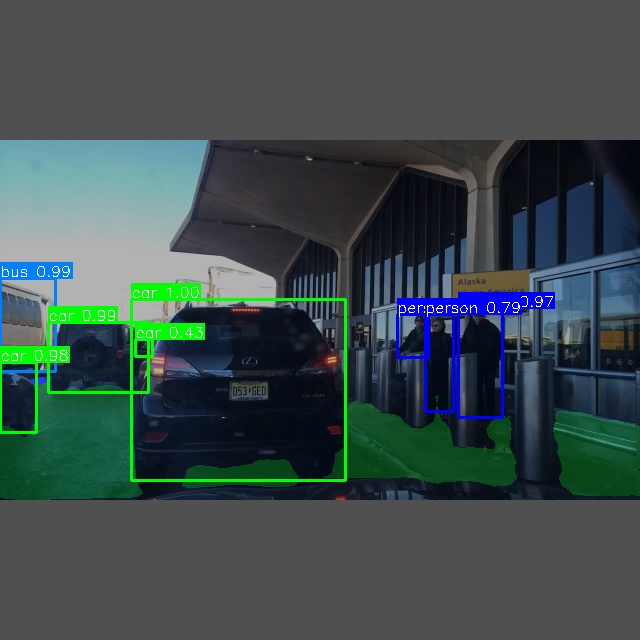
\includegraphics[width=\linewidth]{visualizations/vis_00388_1710645f-b36fa2e7.jpg}
    \caption{vis\_00388\_1710645f-b36fa2e7.jpg}
\end{subfigure}\hfill
\begin{subfigure}[t]{0.32\textwidth}
    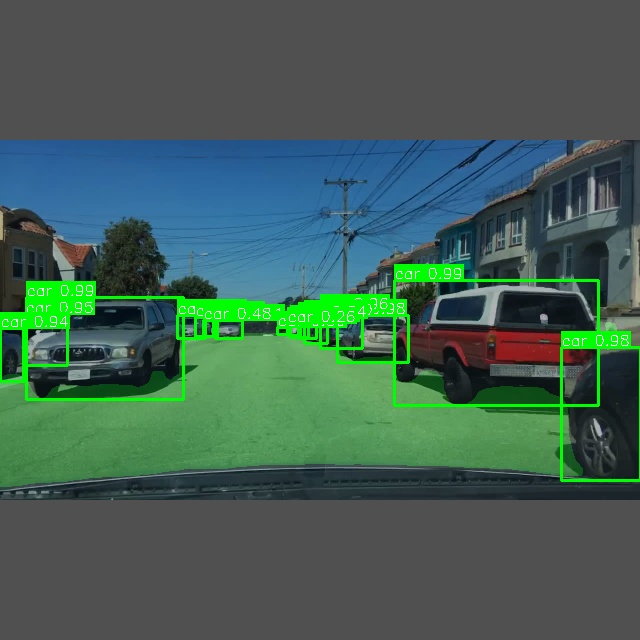
\includegraphics[width=\linewidth]{visualizations/vis_00404_17da591c-7bccf941.jpg}
    \caption{vis\_00404\_17da591c-7bccf941.jpg}
\end{subfigure}\hfill
\begin{subfigure}[t]{0.32\textwidth}
    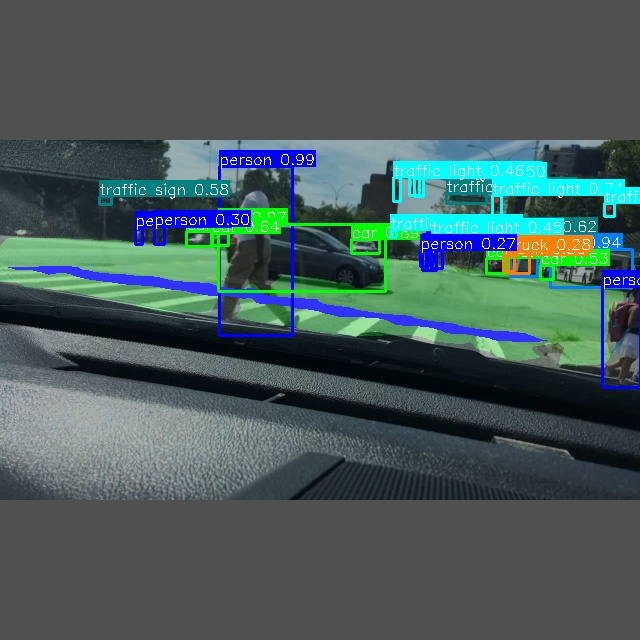
\includegraphics[width=\linewidth]{visualizations/vis_00412_1880e817-8186d9a4.jpg}
    \caption{vis\_00412\_1880e817-8186d9a4.jpg}
\end{subfigure}\hfill
\caption{Six random test images. Each shows boxes + drivable-area mask + lane-line mask overlaid in a single forward pass.}
\label{fig:random-samples}
\end{figure}

\section{Challenging Conditions}

Three subsets carved out of the BDD100K attribute metadata stress-test the model under harder conditions.

\begin{table}[H]
\centering
\caption{Challenging-condition subsets used for qualitative evaluation.}
\label{tab:challenging}
\small
\begin{tabular}{@{}lccl@{}}
\toprule
\textbf{Category} & \textbf{Matched} & \textbf{Saved} & \textbf{Filter} \\
\midrule
Night    & 137 & 12 & \texttt{attributes.timeofday == "night"} \\
Rain     & 253 & 12 & \texttt{attributes.weather == "rainy"} \\
Crowded  & 372 & 12 & $\geq 33$ GT boxes per frame \\
\bottomrule
\end{tabular}
\end{table}

\subsection*{Night Driving}
\begin{figure}[H]
\centering
\begin{subfigure}[t]{0.48\textwidth}
    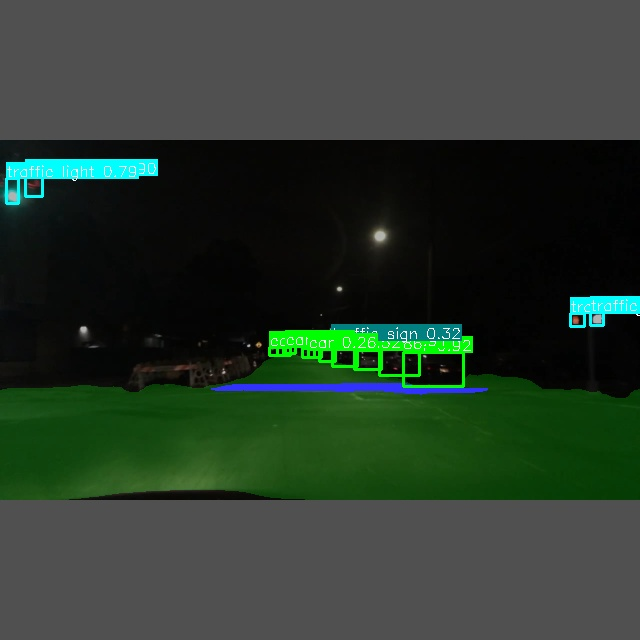
\includegraphics[width=\linewidth]{visualizations/challenging_conditions/night/night_00007_0096bcca-c2027ec4.jpg}
    \caption{night\_00007\_0096bcca-c2027ec4.jpg}
\end{subfigure}\hfill
\begin{subfigure}[t]{0.48\textwidth}
    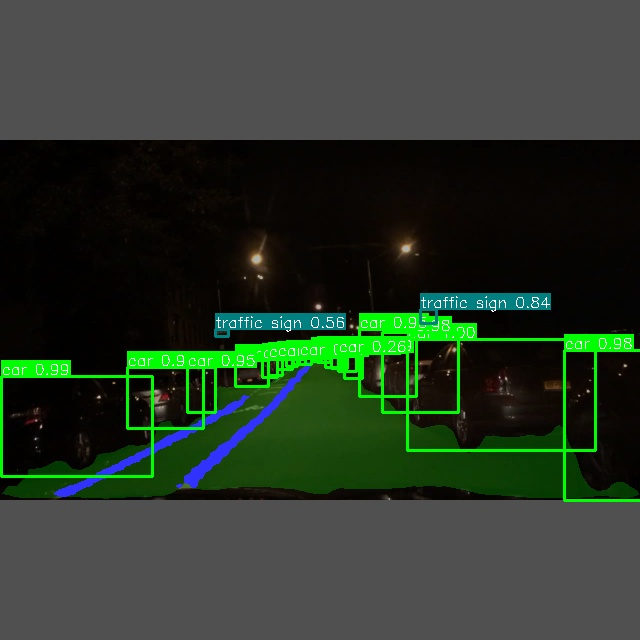
\includegraphics[width=\linewidth]{visualizations/challenging_conditions/night/night_00126_087f969b-b1584c3f.jpg}
    \caption{night\_00126\_087f969b-b1584c3f.jpg}
\end{subfigure}\\[0.4em]
\begin{subfigure}[t]{0.48\textwidth}
    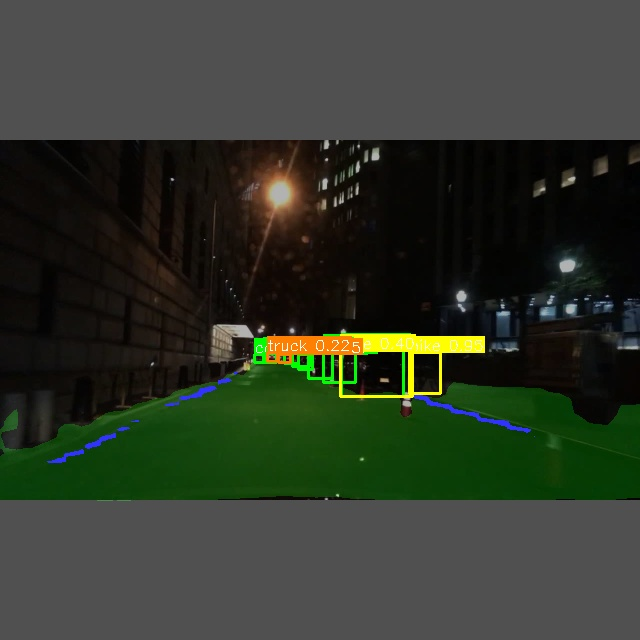
\includegraphics[width=\linewidth]{visualizations/challenging_conditions/night/night_00463_1bf6d50e-48ea2889.jpg}
    \caption{night\_00463\_1bf6d50e-48ea2889.jpg}
\end{subfigure}\hfill
\begin{subfigure}[t]{0.48\textwidth}
    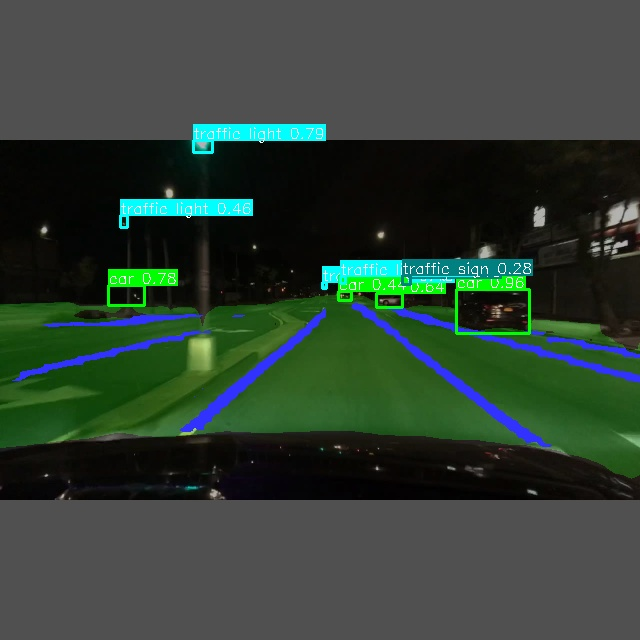
\includegraphics[width=\linewidth]{visualizations/challenging_conditions/night/night_00729_2c917da8-883da6b6.jpg}
    \caption{night\_00729\_2c917da8-883da6b6.jpg}
\end{subfigure}\hfill
\caption{Night Driving subset, four representative frames. Source directory: \texttt{visualizations/challenging\_conditions/night/}.}
\label{fig:night}
\end{figure}
\subsection*{Rainy Weather}
\begin{figure}[H]
\centering
\begin{subfigure}[t]{0.48\textwidth}
    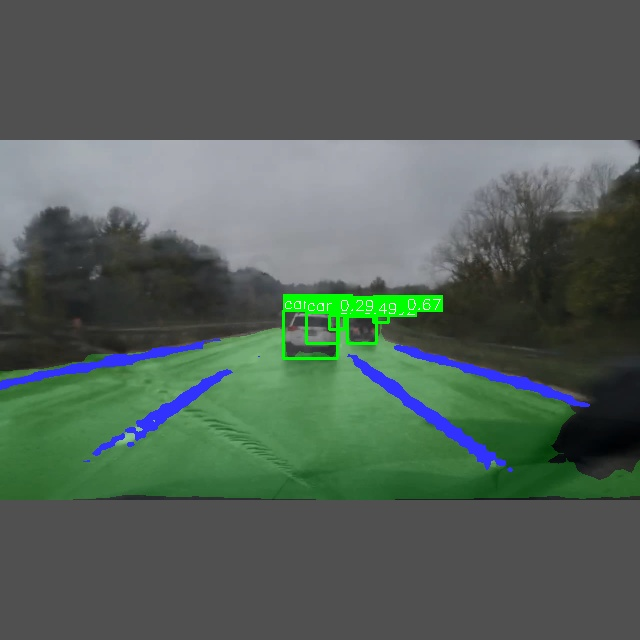
\includegraphics[width=\linewidth]{visualizations/challenging_conditions/rain/rain_00282_11409559-f3c4582b.jpg}
    \caption{rain\_00282\_11409559-f3c4582b.jpg}
\end{subfigure}\hfill
\begin{subfigure}[t]{0.48\textwidth}
    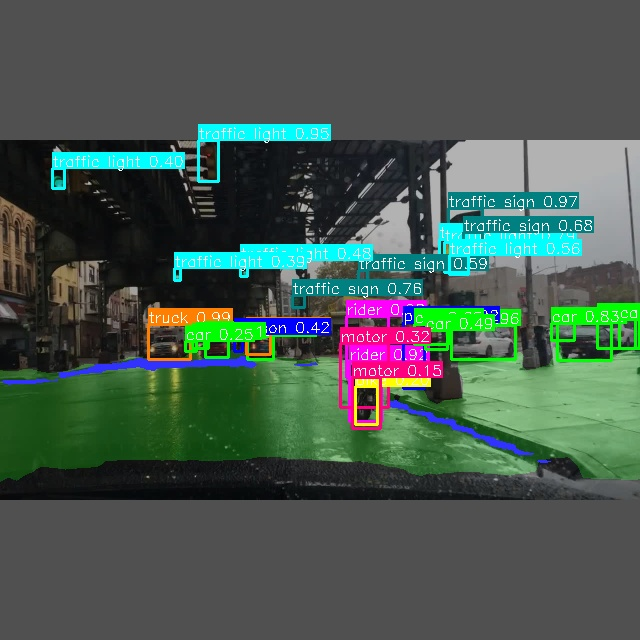
\includegraphics[width=\linewidth]{visualizations/challenging_conditions/rain/rain_00314_13163948-7d0574d6.jpg}
    \caption{rain\_00314\_13163948-7d0574d6.jpg}
\end{subfigure}\\[0.4em]
\begin{subfigure}[t]{0.48\textwidth}
    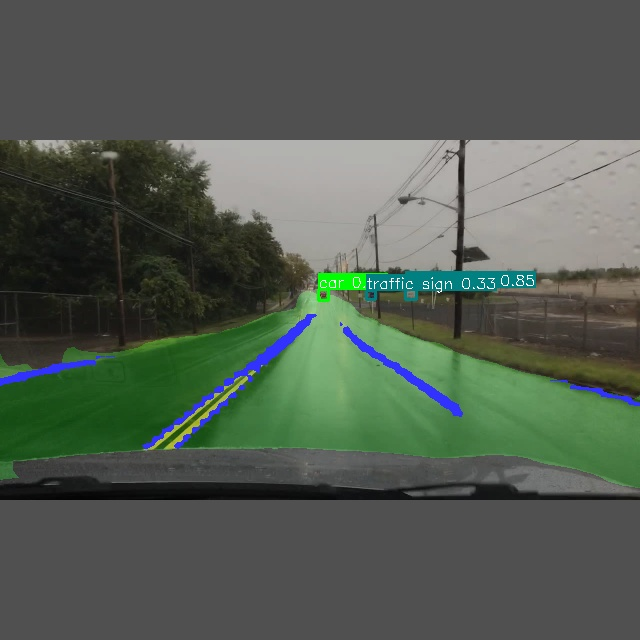
\includegraphics[width=\linewidth]{visualizations/challenging_conditions/rain/rain_00447_1a760b64-33c25ec5.jpg}
    \caption{rain\_00447\_1a760b64-33c25ec5.jpg}
\end{subfigure}\hfill
\begin{subfigure}[t]{0.48\textwidth}
    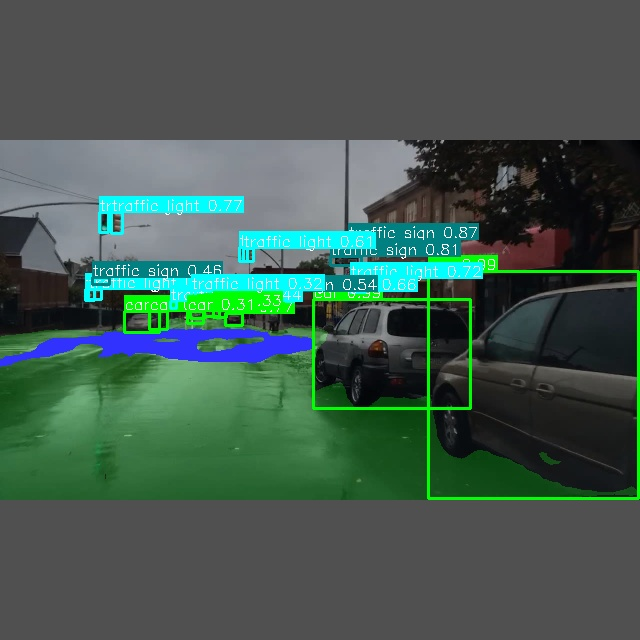
\includegraphics[width=\linewidth]{visualizations/challenging_conditions/rain/rain_01189_475a4732-7fd6ed1d.jpg}
    \caption{rain\_01189\_475a4732-7fd6ed1d.jpg}
\end{subfigure}\hfill
\caption{Rainy Weather subset, four representative frames. Source directory: \texttt{visualizations/challenging\_conditions/rain/}.}
\label{fig:rain}
\end{figure}
\subsection*{Crowded Scenes ($\geq 33$ GT boxes)}
\begin{figure}[H]
\centering
\begin{subfigure}[t]{0.48\textwidth}
    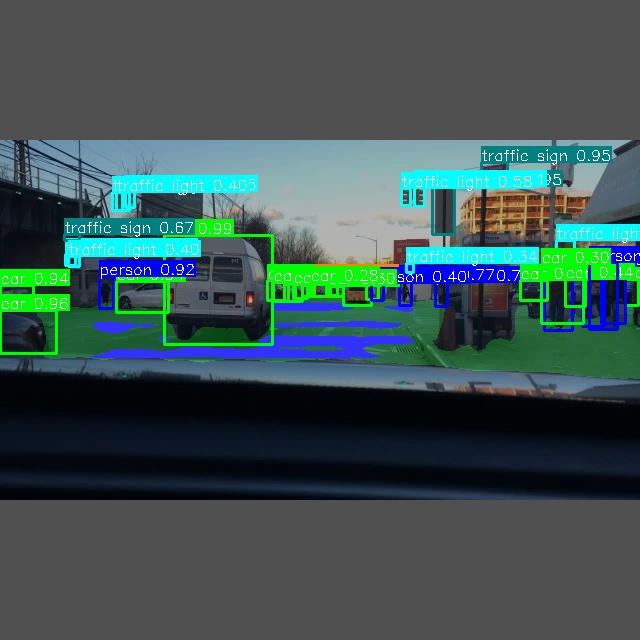
\includegraphics[width=\linewidth]{visualizations/challenging_conditions/crowded/crowded_00522_1faaee6b-c0b27c70.jpg}
    \caption{crowded\_00522\_1faaee6b-c0b27c70.jpg}
\end{subfigure}\hfill
\begin{subfigure}[t]{0.48\textwidth}
    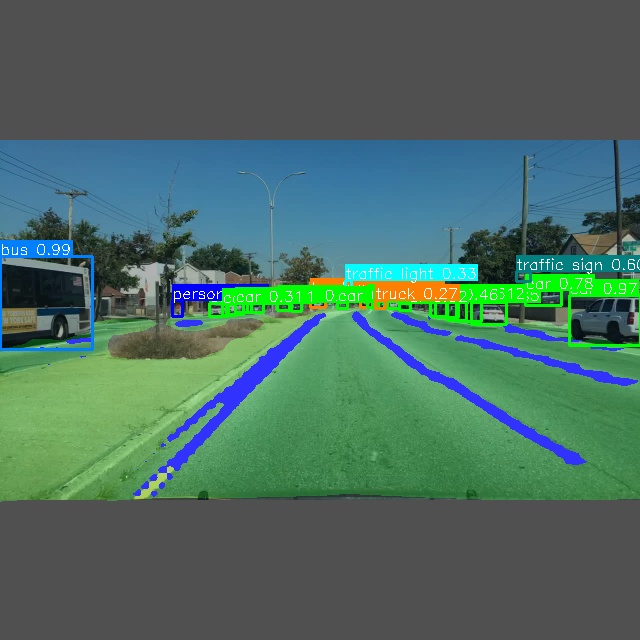
\includegraphics[width=\linewidth]{visualizations/challenging_conditions/crowded/crowded_00606_242f73d4-325f020c.jpg}
    \caption{crowded\_00606\_242f73d4-325f020c.jpg}
\end{subfigure}\\[0.4em]
\begin{subfigure}[t]{0.48\textwidth}
    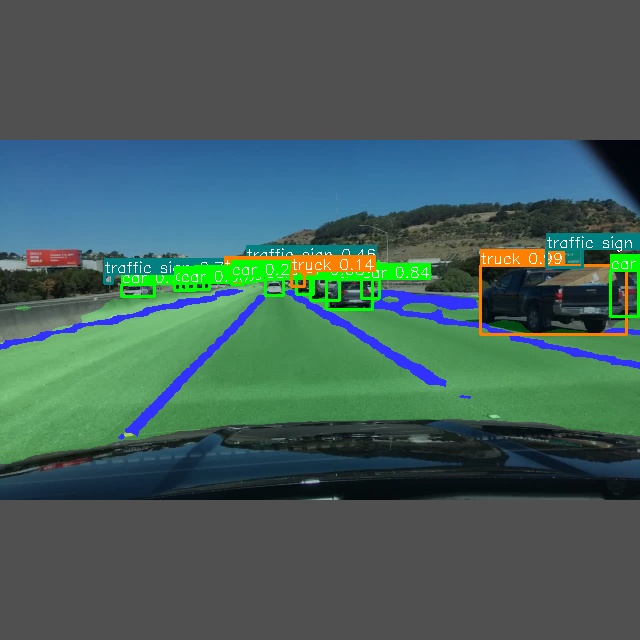
\includegraphics[width=\linewidth]{visualizations/challenging_conditions/crowded/crowded_00944_388af398-d6141a4c.jpg}
    \caption{crowded\_00944\_388af398-d6141a4c.jpg}
\end{subfigure}\hfill
\begin{subfigure}[t]{0.48\textwidth}
    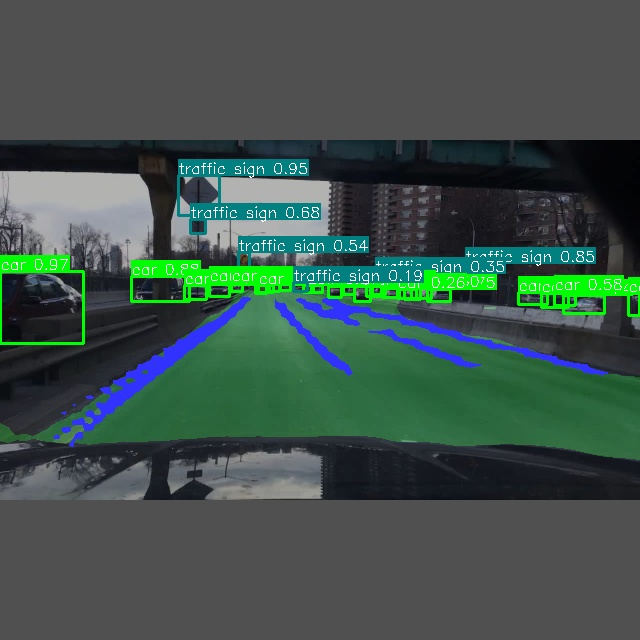
\includegraphics[width=\linewidth]{visualizations/challenging_conditions/crowded/crowded_01440_575a2428-b724fc19.jpg}
    \caption{crowded\_01440\_575a2428-b724fc19.jpg}
\end{subfigure}\hfill
\caption{Crowded Scenes ($\geq 33$ GT boxes) subset, four representative frames. Source directory: \texttt{visualizations/challenging\_conditions/crowded/}.}
\label{fig:crowded}
\end{figure}

\section{Hard Examples (Highest Multi-Task Loss)}

We rank the labelled test set by per-image multi-task loss (detection + drivable + lane). These are the frames where the model struggles the most, typically combining dense small targets, ambiguous lane markings, and low-light or weather effects.

\begin{figure}[H]
\centering
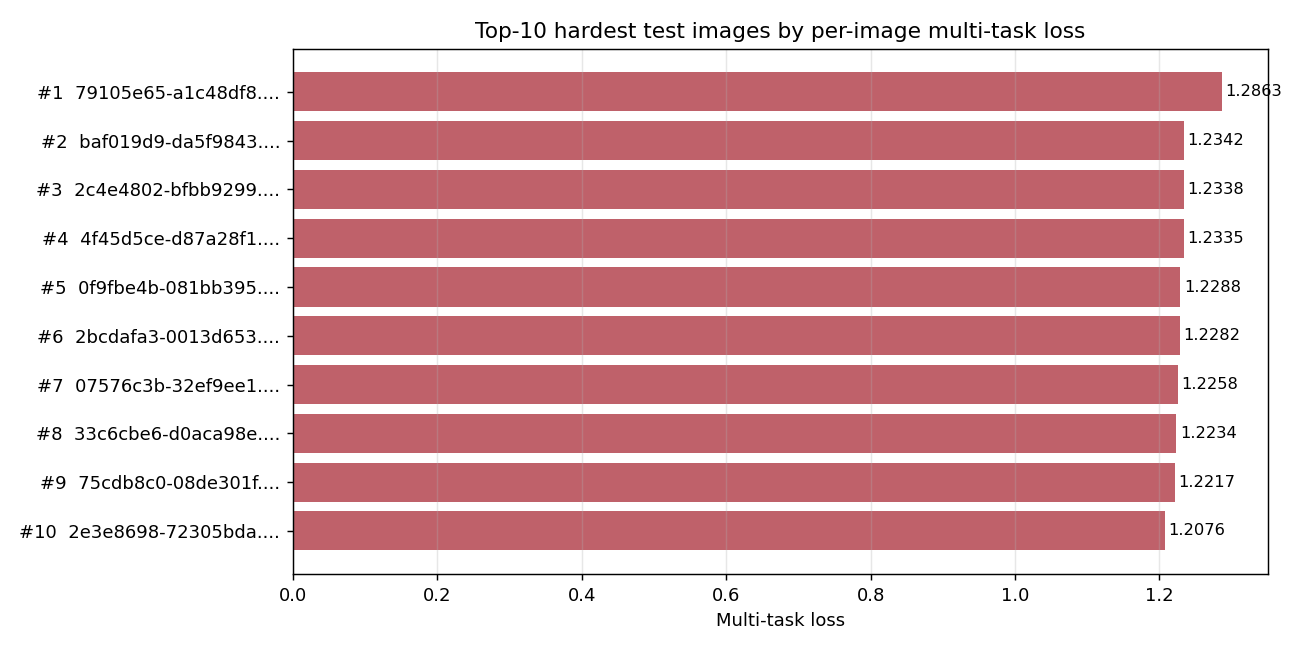
\includegraphics[width=0.88\textwidth]{plots/hard_example_losses.png}
\caption{Top-10 hardest test images by total multi-task loss. Loss values cluster between $1.21$ and $1.29$.}
\label{fig:hard-loss-bar}
\end{figure}

\begin{figure}[H]
\centering
\begin{subfigure}[t]{0.48\textwidth}
    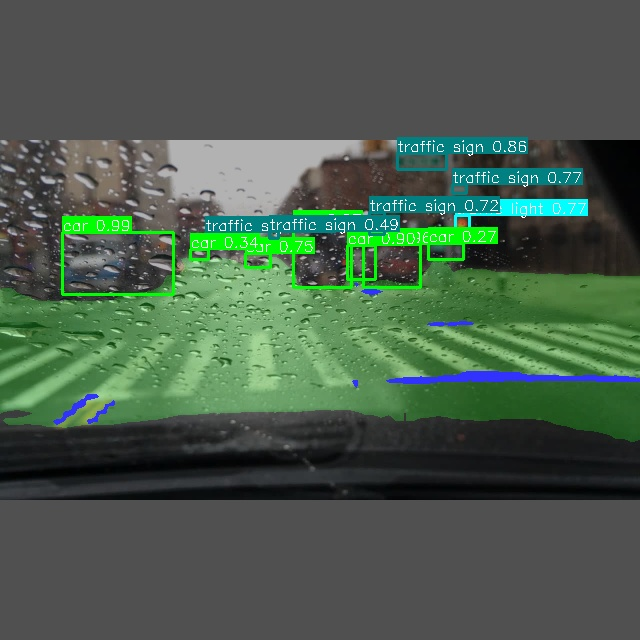
\includegraphics[width=\linewidth]{hard_examples/hard_01_79105e65-a1c48df8.jpg}
    \caption{Rank \#1 (loss 1.2863): \texttt{79105e65-a1c48df8.jpg}}
\end{subfigure}\hfill
\begin{subfigure}[t]{0.48\textwidth}
    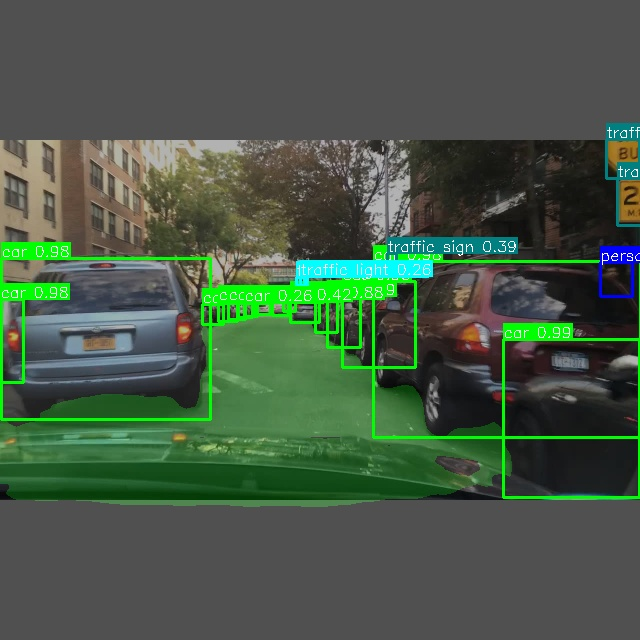
\includegraphics[width=\linewidth]{hard_examples/hard_02_baf019d9-da5f9843.jpg}
    \caption{Rank \#2 (loss 1.2342): \texttt{baf019d9-da5f9843.jpg}}
\end{subfigure}
\caption{Hard examples 1--2 by multi-task loss. Source: \texttt{runs/test/hard\_examples/}.}
\label{fig:hard-1}
\end{figure}
\begin{figure}[H]
\centering
\begin{subfigure}[t]{0.48\textwidth}
    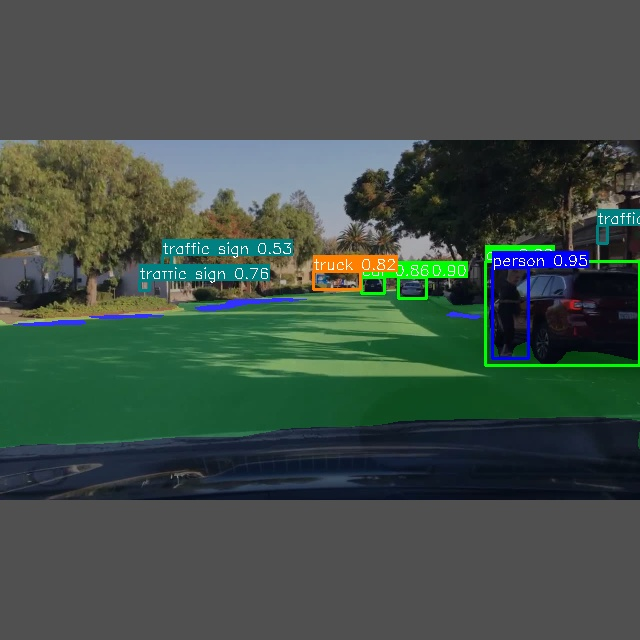
\includegraphics[width=\linewidth]{hard_examples/hard_03_2c4e4802-bfbb9299.jpg}
    \caption{Rank \#3 (loss 1.2338): \texttt{2c4e4802-bfbb9299.jpg}}
\end{subfigure}\hfill
\begin{subfigure}[t]{0.48\textwidth}
    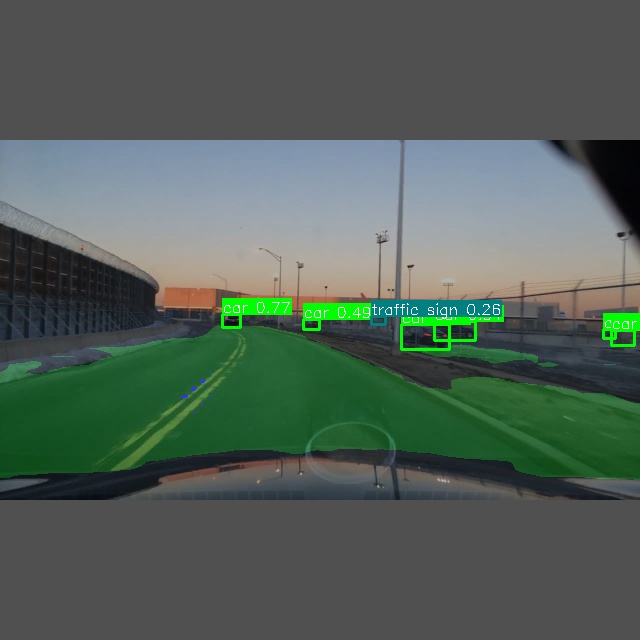
\includegraphics[width=\linewidth]{hard_examples/hard_04_4f45d5ce-d87a28f1.jpg}
    \caption{Rank \#4 (loss 1.2335): \texttt{4f45d5ce-d87a28f1.jpg}}
\end{subfigure}
\caption{Hard examples 3--4 by multi-task loss. Source: \texttt{runs/test/hard\_examples/}.}
\label{fig:hard-2}
\end{figure}
\begin{figure}[H]
\centering
\begin{subfigure}[t]{0.48\textwidth}
    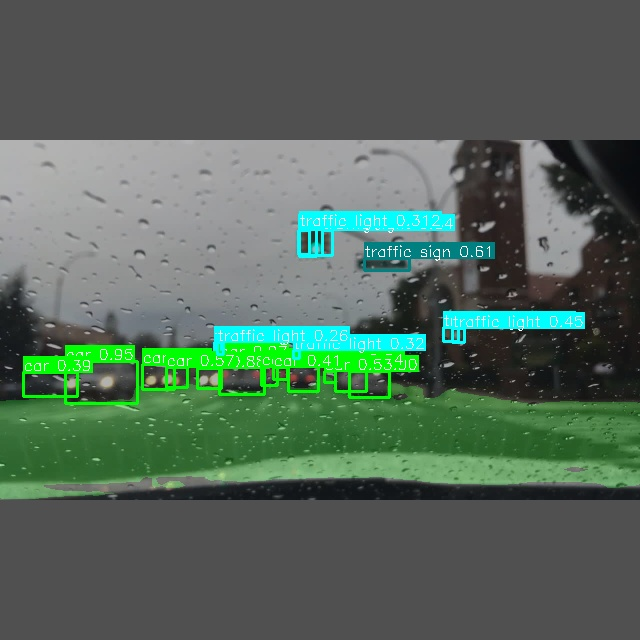
\includegraphics[width=\linewidth]{hard_examples/hard_05_0f9fbe4b-081bb395.jpg}
    \caption{Rank \#5 (loss 1.2288): \texttt{0f9fbe4b-081bb395.jpg}}
\end{subfigure}\hfill
\begin{subfigure}[t]{0.48\textwidth}
    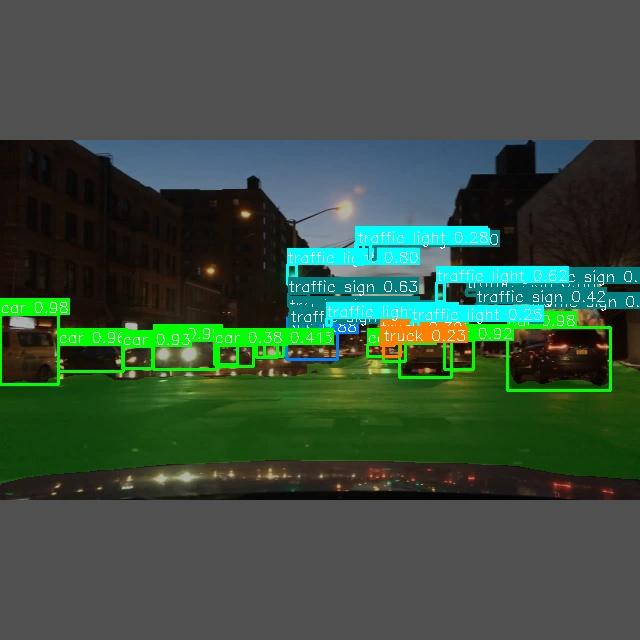
\includegraphics[width=\linewidth]{hard_examples/hard_06_2bcdafa3-0013d653.jpg}
    \caption{Rank \#6 (loss 1.2282): \texttt{2bcdafa3-0013d653.jpg}}
\end{subfigure}
\caption{Hard examples 5--6 by multi-task loss. Source: \texttt{runs/test/hard\_examples/}.}
\label{fig:hard-3}
\end{figure}
\begin{figure}[H]
\centering
\begin{subfigure}[t]{0.48\textwidth}
    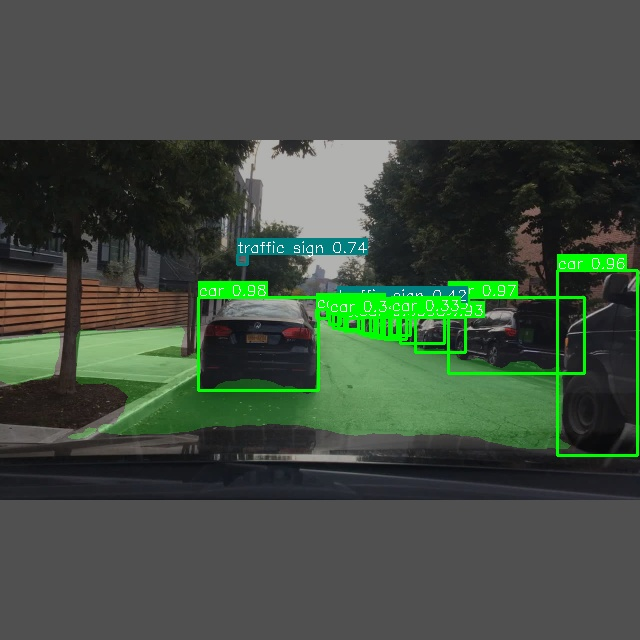
\includegraphics[width=\linewidth]{hard_examples/hard_07_07576c3b-32ef9ee1.jpg}
    \caption{Rank \#7 (loss 1.2258): \texttt{07576c3b-32ef9ee1.jpg}}
\end{subfigure}\hfill
\begin{subfigure}[t]{0.48\textwidth}
    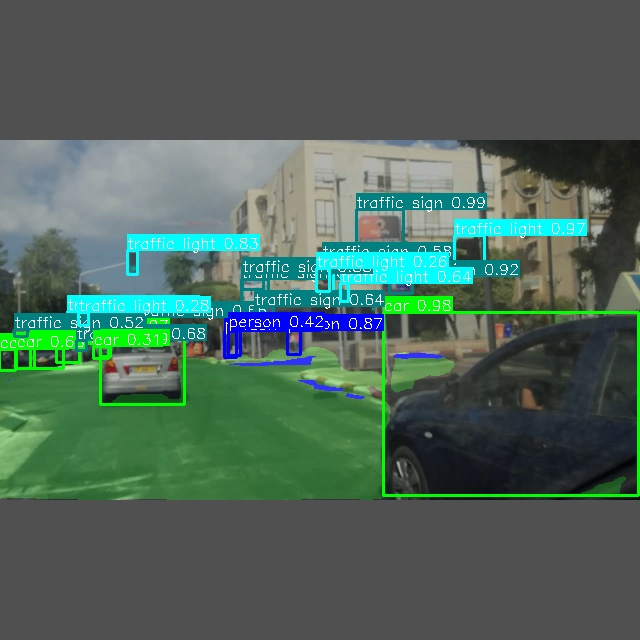
\includegraphics[width=\linewidth]{hard_examples/hard_08_33c6cbe6-d0aca98e.jpg}
    \caption{Rank \#8 (loss 1.2234): \texttt{33c6cbe6-d0aca98e.jpg}}
\end{subfigure}
\caption{Hard examples 7--8 by multi-task loss. Source: \texttt{runs/test/hard\_examples/}.}
\label{fig:hard-4}
\end{figure}
\begin{figure}[H]
\centering
\begin{subfigure}[t]{0.48\textwidth}
    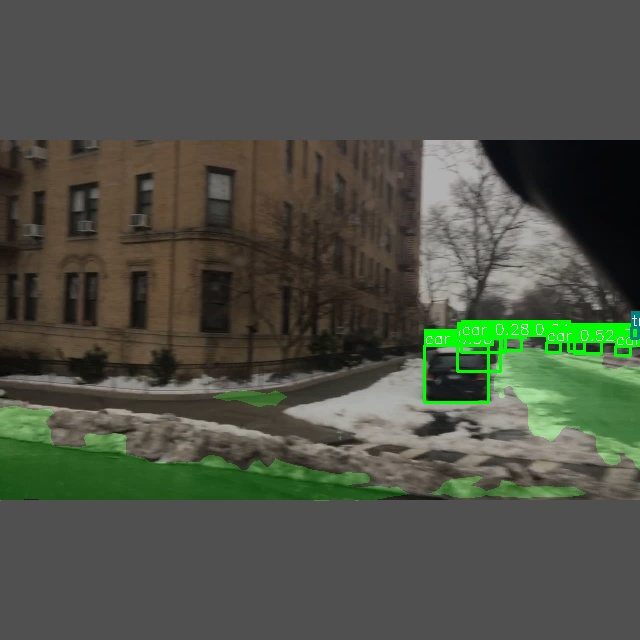
\includegraphics[width=\linewidth]{hard_examples/hard_09_75cdb8c0-08de301f.jpg}
    \caption{Rank \#9 (loss 1.2217): \texttt{75cdb8c0-08de301f.jpg}}
\end{subfigure}\hfill
\begin{subfigure}[t]{0.48\textwidth}
    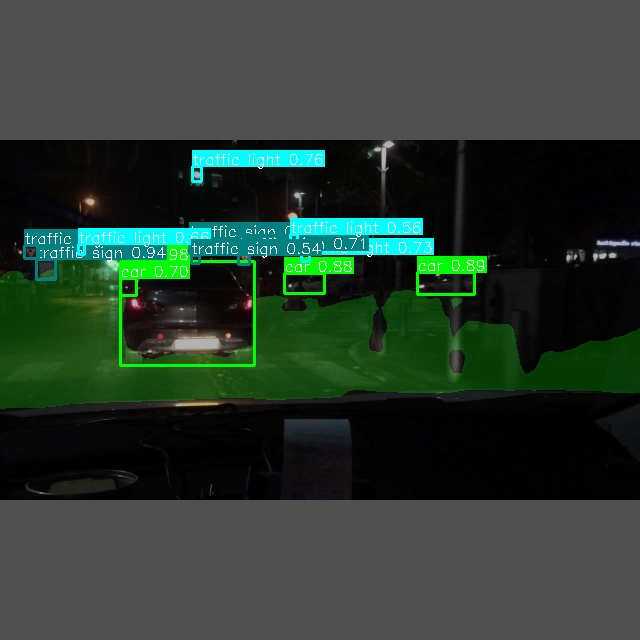
\includegraphics[width=\linewidth]{hard_examples/hard_10_2e3e8698-72305bda.jpg}
    \caption{Rank \#10 (loss 1.2076): \texttt{2e3e8698-72305bda.jpg}}
\end{subfigure}
\caption{Hard examples 9--10 by multi-task loss. Source: \texttt{runs/test/hard\_examples/}.}
\label{fig:hard-5}
\end{figure}

\section{Lane-Line Diagnostic Panels}

Each panel is a four-up view, left to right: \textbf{original frame} $|$ \textbf{ground-truth lane mask} $|$ \textbf{predicted sigmoid heatmap} $|$ \textbf{thresholded prediction at $0.5$}. The heatmap aligns with real lane boundaries, crosswalks, and stop bars, confirming that the lane head produces meaningful spatial signal rather than noise. These panels are the direct IoU-related diagnostic, showing exactly where the model's predicted mask matches and where it misses the thin polyline ground truth.

\begin{figure}[H]
\centering
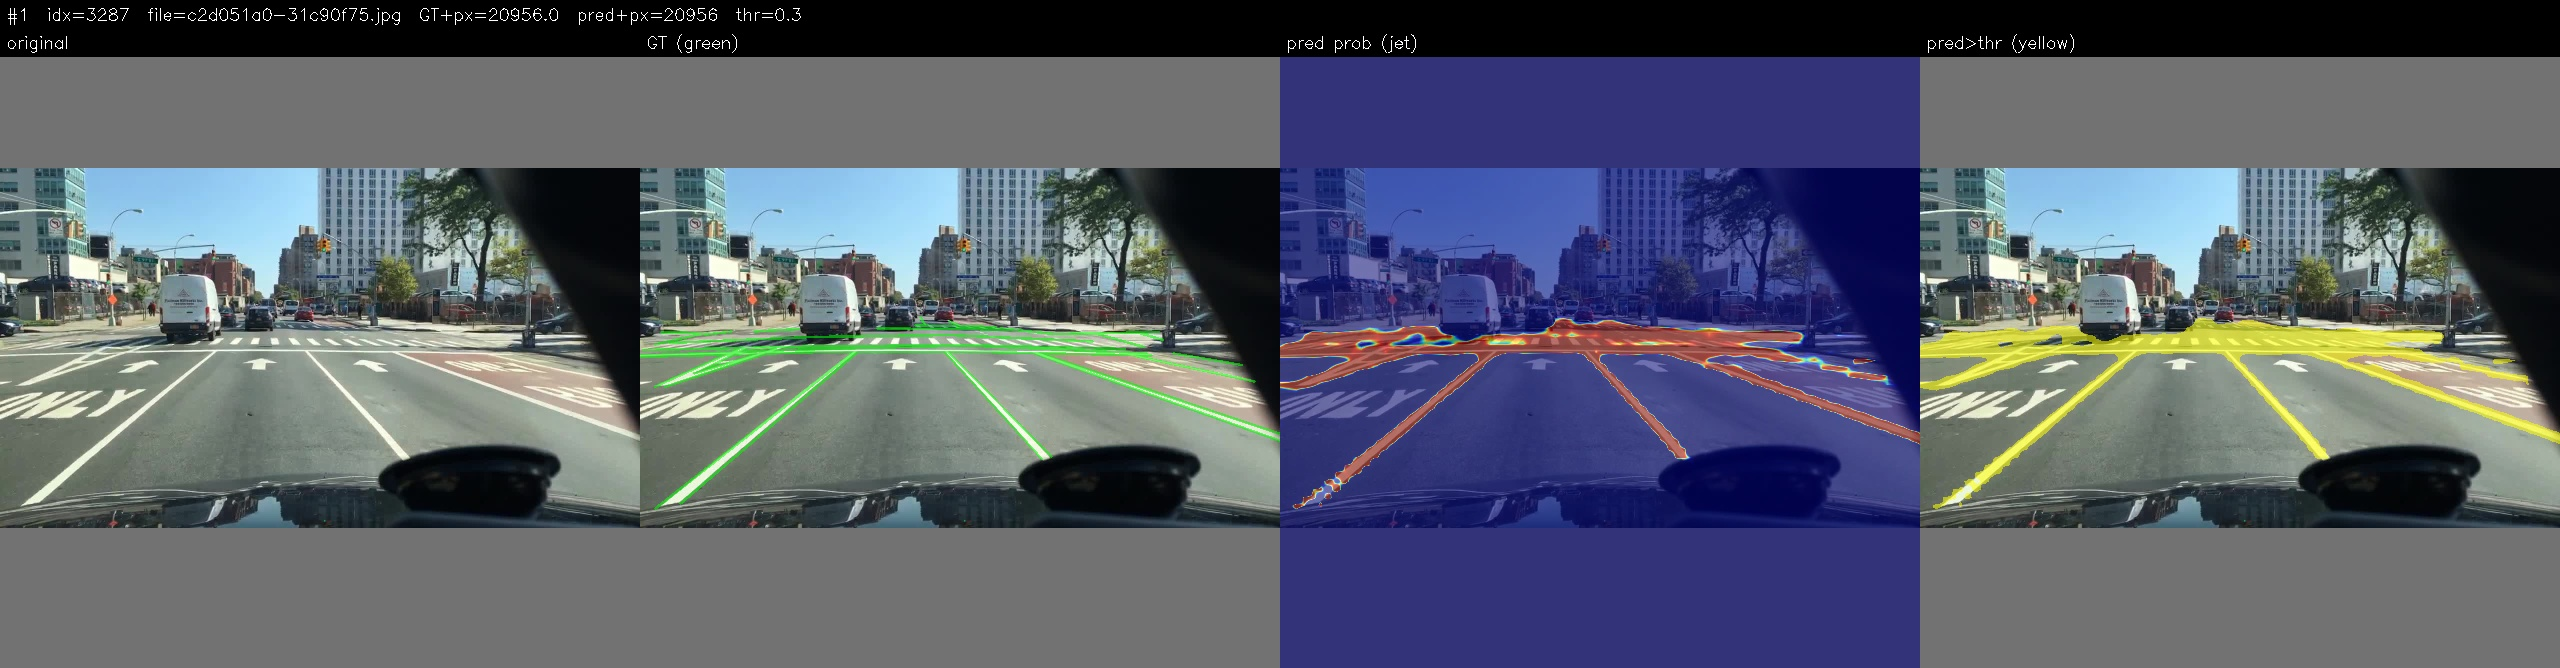
\includegraphics[width=\textwidth]{ll_diagnostics/panels/panel_01_idx3287.jpg}
\caption{Lane-line diagnostic panel \texttt{panel\_01\_idx3287.jpg}. Columns: original frame $|$ GT lane mask $|$ predicted heatmap $|$ thresholded prediction.}
\label{fig:ll-panel-1}
\end{figure}
\begin{figure}[H]
\centering
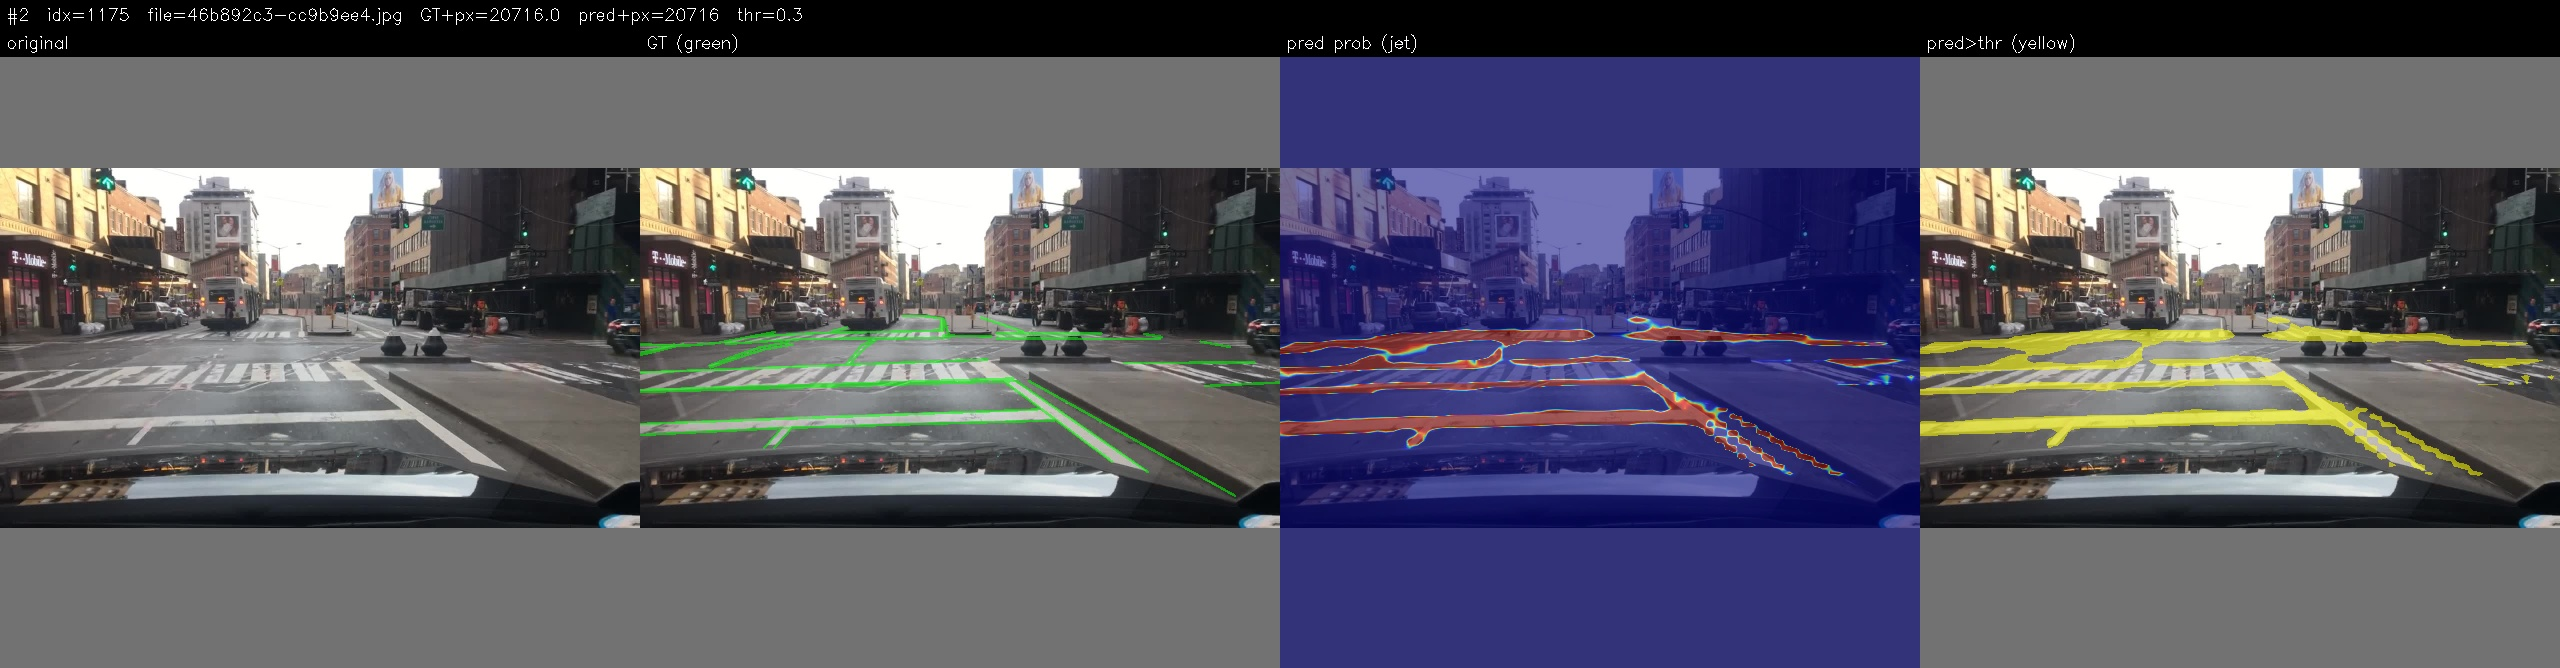
\includegraphics[width=\textwidth]{ll_diagnostics/panels/panel_02_idx1175.jpg}
\caption{Lane-line diagnostic panel \texttt{panel\_02\_idx1175.jpg}. Columns: original frame $|$ GT lane mask $|$ predicted heatmap $|$ thresholded prediction.}
\label{fig:ll-panel-2}
\end{figure}
\begin{figure}[H]
\centering
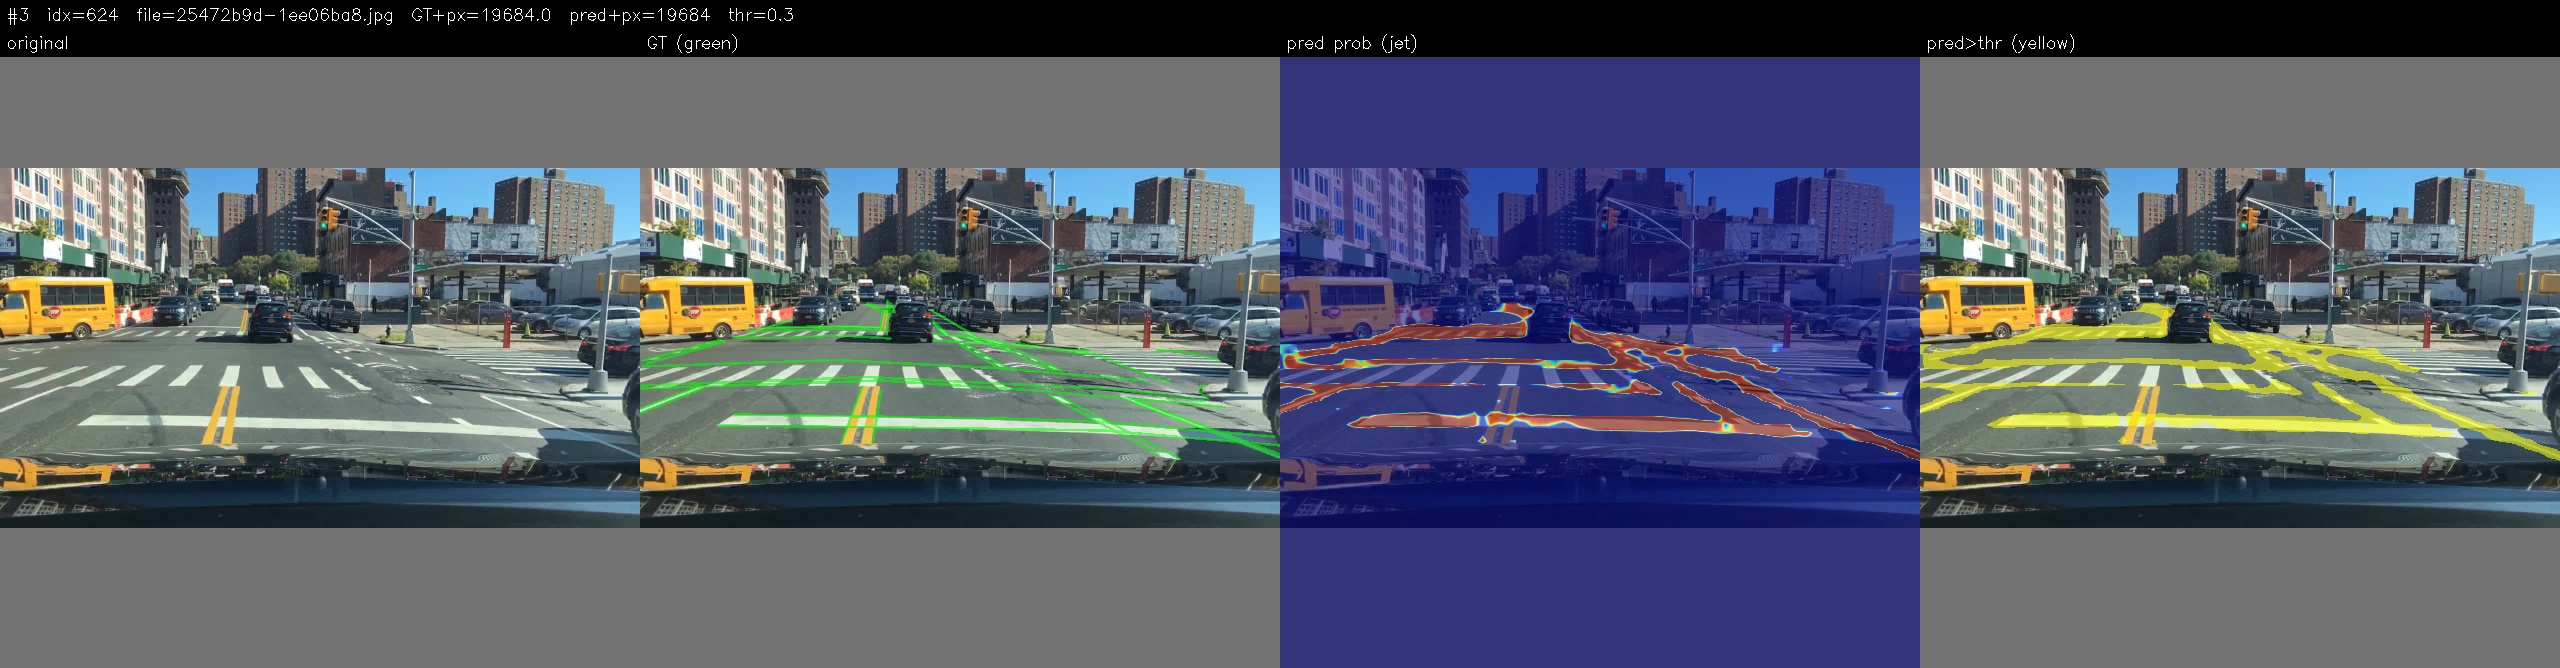
\includegraphics[width=\textwidth]{ll_diagnostics/panels/panel_03_idx0624.jpg}
\caption{Lane-line diagnostic panel \texttt{panel\_03\_idx0624.jpg}. Columns: original frame $|$ GT lane mask $|$ predicted heatmap $|$ thresholded prediction.}
\label{fig:ll-panel-3}
\end{figure}
\begin{figure}[H]
\centering
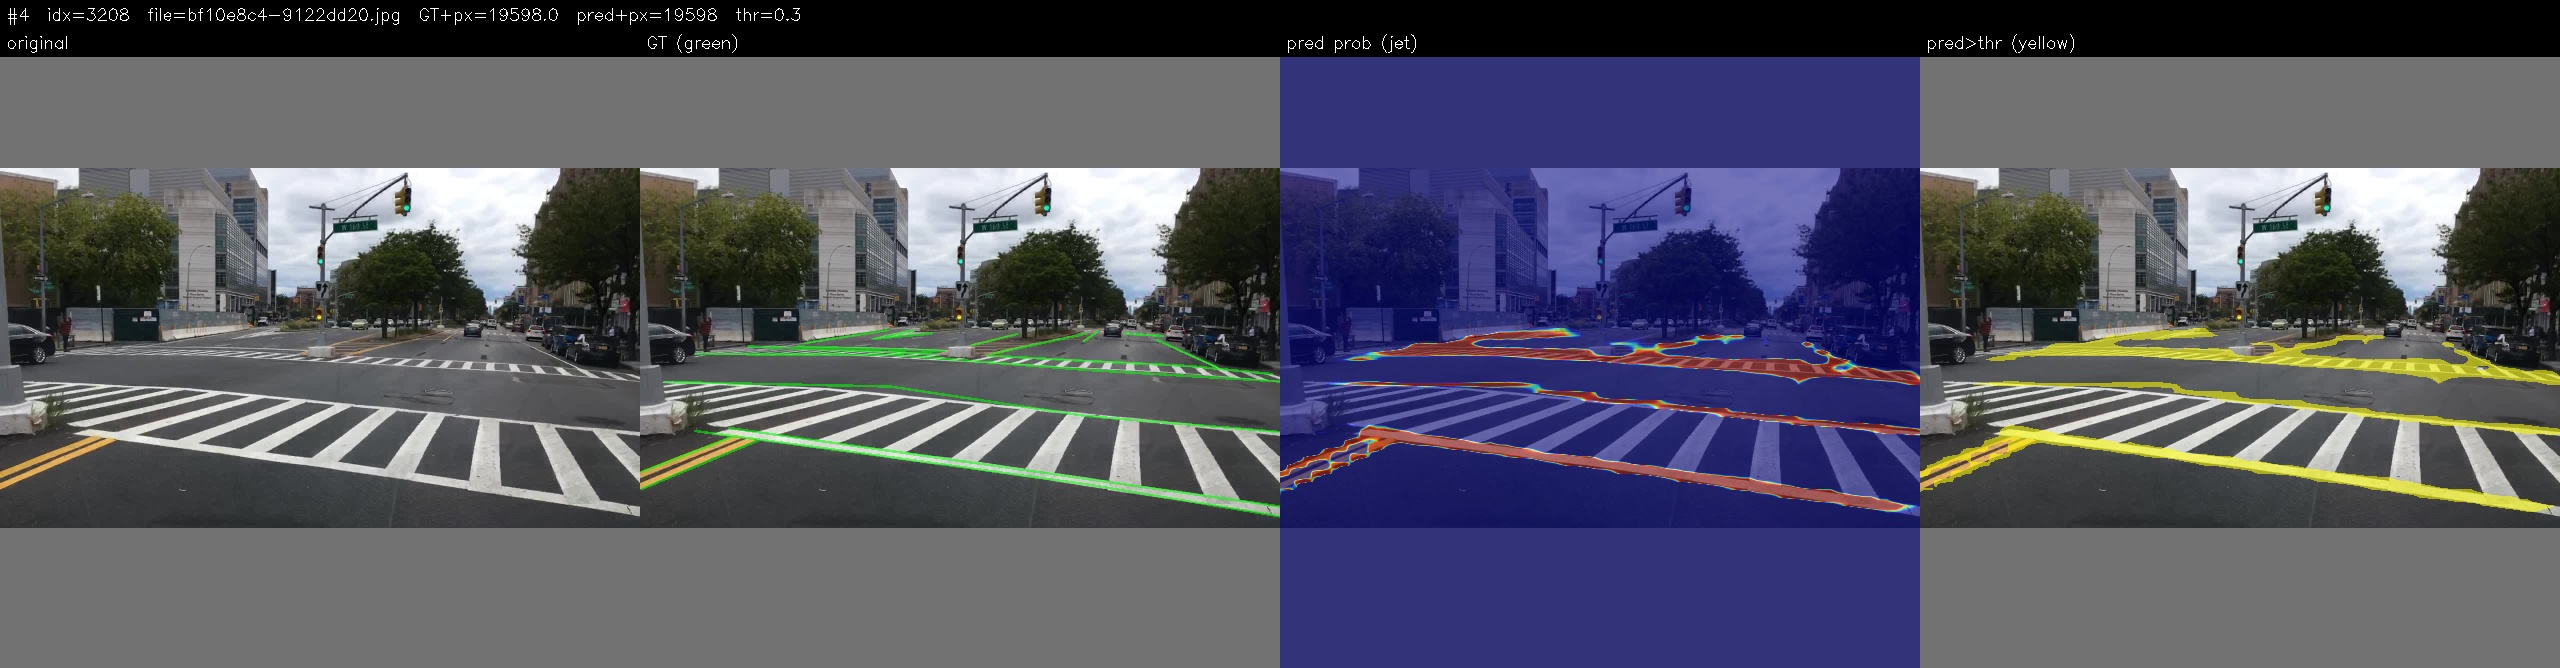
\includegraphics[width=\textwidth]{ll_diagnostics/panels/panel_04_idx3208.jpg}
\caption{Lane-line diagnostic panel \texttt{panel\_04\_idx3208.jpg}. Columns: original frame $|$ GT lane mask $|$ predicted heatmap $|$ thresholded prediction.}
\label{fig:ll-panel-4}
\end{figure}
\begin{figure}[H]
\centering
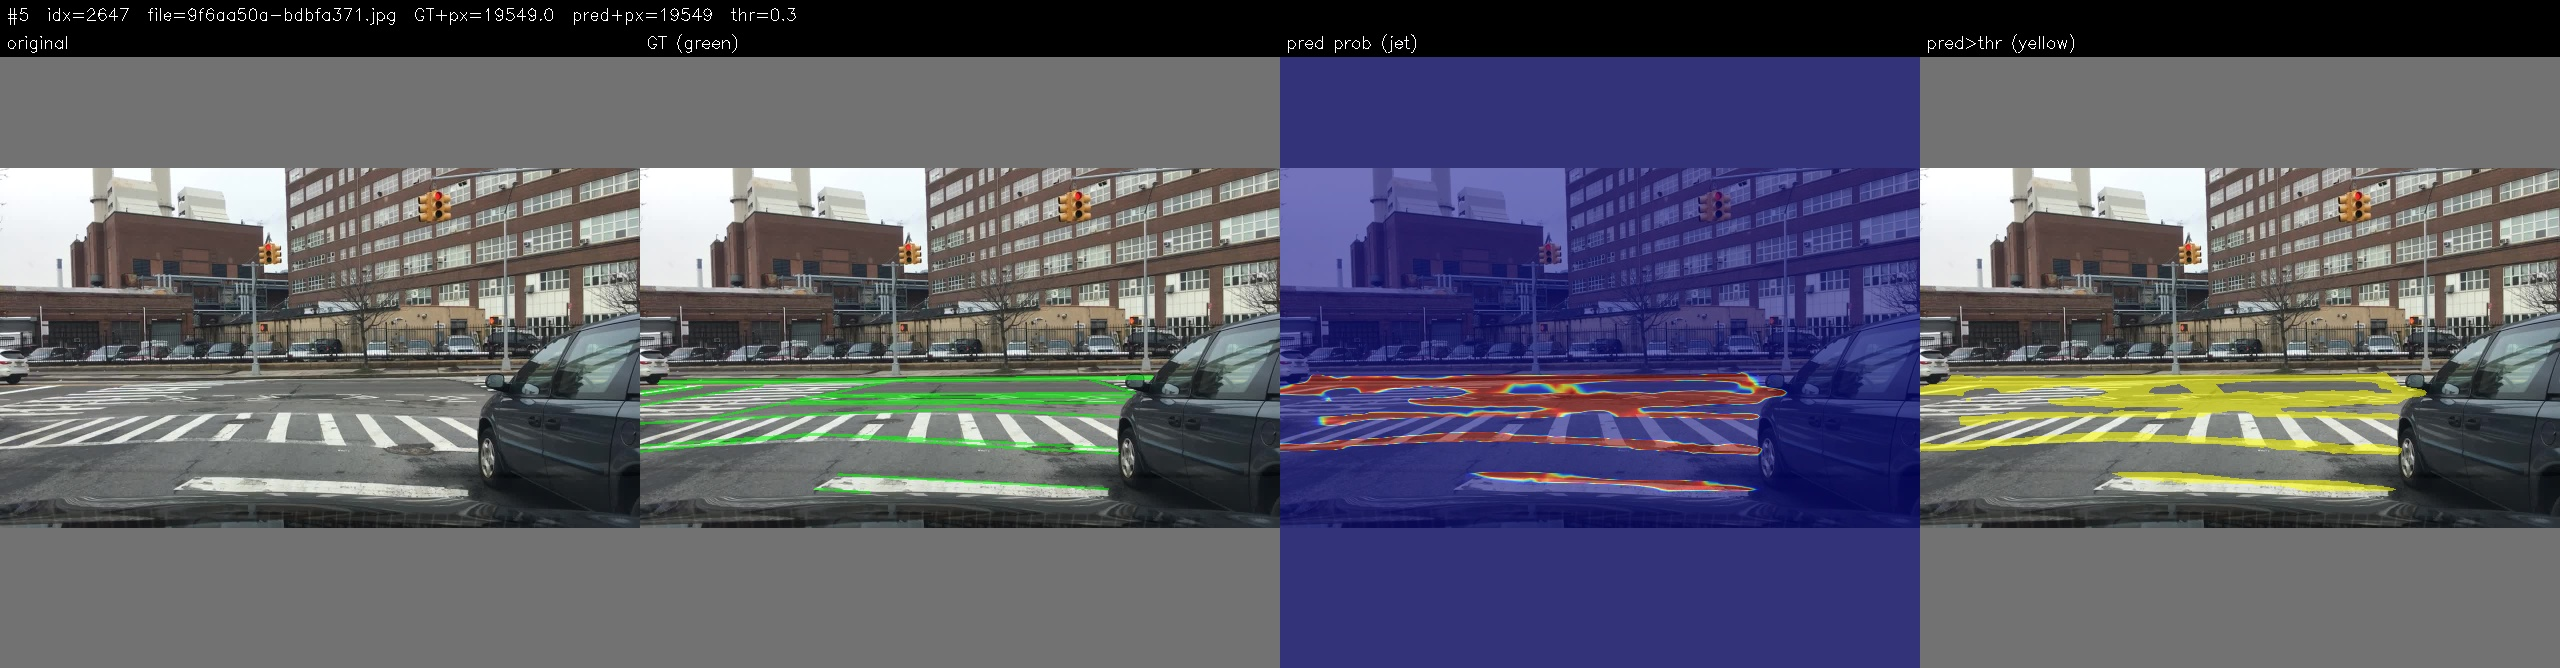
\includegraphics[width=\textwidth]{ll_diagnostics/panels/panel_05_idx2647.jpg}
\caption{Lane-line diagnostic panel \texttt{panel\_05\_idx2647.jpg}. Columns: original frame $|$ GT lane mask $|$ predicted heatmap $|$ thresholded prediction.}
\label{fig:ll-panel-5}
\end{figure}
\begin{figure}[H]
\centering
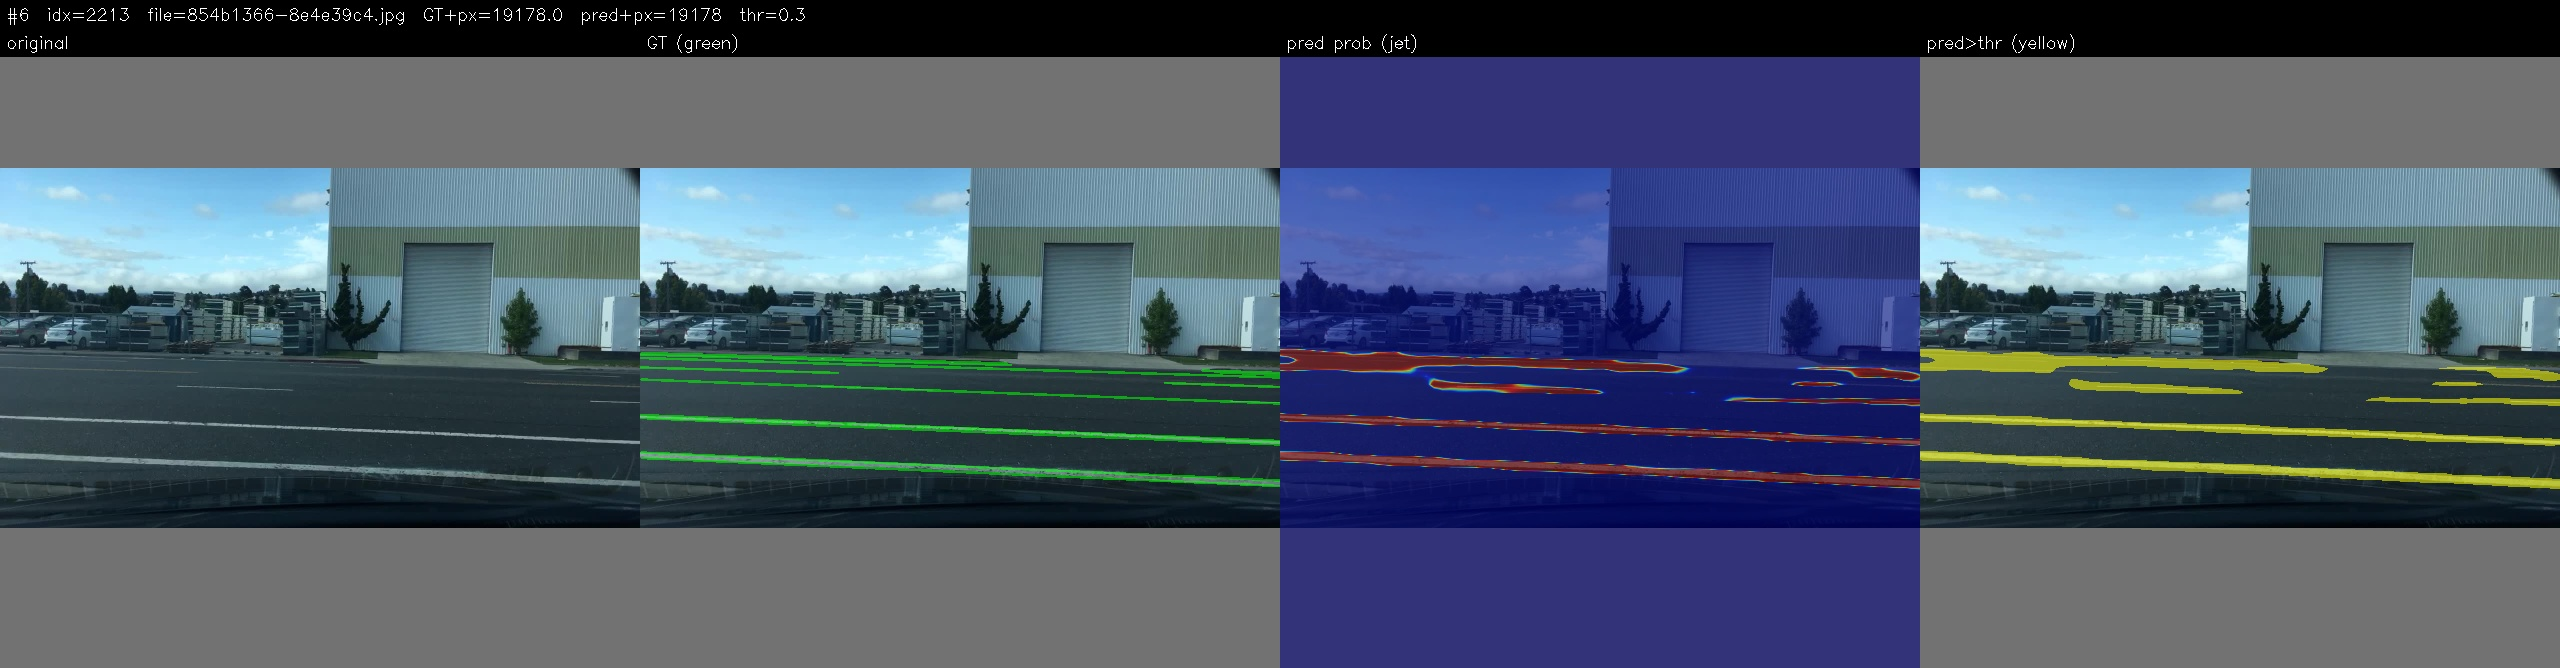
\includegraphics[width=\textwidth]{ll_diagnostics/panels/panel_06_idx2213.jpg}
\caption{Lane-line diagnostic panel \texttt{panel\_06\_idx2213.jpg}. Columns: original frame $|$ GT lane mask $|$ predicted heatmap $|$ thresholded prediction.}
\label{fig:ll-panel-6}
\end{figure}

\chapter{Conclusion}

The progression through R-CNN, Faster R-CNN, YOLOv8, and YOLOPv2 traces a familiar pattern. Each step trades a small accuracy concession for a large efficiency gain, then claws the accuracy back through better losses, schedules, and label sets.

The two-stage detectors served as instructive baselines. R-CNN demonstrated the principle. Faster R-CNN refined it into something accurate enough for offline analytics on a single-class problem. Neither met the latency budget for live video. YOLOv8 closed the latency gap, but detection-only output still demands a second network for segmentation.

YOLOPv2 collapses three networks into one forward pass. On the BDD100K labelled subset it returns ten-class detections at mAP@0.5 $= 0.676$ (vehicle subset $0.83$), drivable-area mIoU $0.95$, and lane-line mIoU $0.69$, at $206$ FPS on a single RTX 6000 Ada at batch 1 and $477$ FPS at batch 4. The model weighs $23.4$~M parameters. Training was stable across 100 epochs with monotonic descent on every loss component.

For analysing traffic hubs and commuter patterns, the throughput is the headline result. A pipeline built on this model can process a $30$-FPS camera feed and still have over an order of magnitude of compute headroom for tracking, motion estimation, and per-vehicle attribute extraction. The multi-task structure delivers three structured output layers per frame for the cost of one. That combination is what a real traffic-flow estimator needs at the input stage.

Two extensions are worth flagging. A genuine held-out split, carved out before training, would convert the current training-fit numbers into proper generalisation estimates. A temporal head fusing two or three consecutive frames would let the downstream tracker share work with the detector rather than redoing it on every frame. Both are achievable on top of the present pipeline.

\appendix

\chapter{Reproduction Commands}

\begin{lstlisting}[language=bash]
# Full evaluation: mAP, P/R/F1, segmentation, hard examples
CUDA_VISIBLE_DEVICES=4 python evaluate.py \
    --weights runs/train/last.pt --data-root ../bdd100k_data \
    --split train --require-labels \
    --batch-size 8 --num-vis 0 --num-hard 10 --output-dir runs/test

# LL threshold sweep + diagnostic panels
CUDA_VISIBLE_DEVICES=4 python diagnose_ll.py \
    --weights runs/train/last.pt --data-root ../bdd100k_data \
    --split train --require-labels \
    --thresholds 0.1,0.2,0.3,0.4,0.5 --num-panels 12 \
    --output-dir runs/test/ll_diagnostics

# Real-time benchmark
CUDA_VISIBLE_DEVICES=4 python benchmark.py \
    --weights runs/train/last.pt --n-iters 100 \
    --batch-sizes 1,4,8,16,32 --output runs/test/benchmark.json

# Reconstruct training loss curves from saved checkpoints
CUDA_VISIBLE_DEVICES=4 python recover_train_curves.py \
    --ckpt-dir runs/train --data-root ../bdd100k_data \
    --batch-size 8 --n-samples 320 --output-dir runs/test/plots

# Random + challenging-condition visualizations
CUDA_VISIBLE_DEVICES=4 python visualize_challenging.py \
    --weights runs/train/last.pt --data-root ../bdd100k_data \
    --num-random 50 --per-category 12 \
    --output-root runs/test/visualizations

# Build analysis charts and reports
python build_charts.py
python build_report.py
python build_latex_report.py
\end{lstlisting}

\end{document}
